\documentclass[9pt,a4paper,unknownkeysallowed,xcolor=dvipsnames,aspectratio=43]{beamer}
\usepackage[percent]{overpic}
%aspectratio=1610, 169, 149, 54, 43 and 32
\usepackage{subfigure,graphicx}
\usepackage{hyperref}  
\usepackage{pifont}
%\setbeamertemplate{footline}{\centerline{\fontsize{6pt}{1em}\it { \thepage}}} 
%\usetheme{Copenhagen}
\usepackage{ifthen}
\usepackage{bm,amsmath,amssymb}
\usepackage[mathscr]{eucal}
\usepackage{epsfig}
\usepackage{graphicx}
\usepackage{CJK}
\usepackage[percent]{overpic}
\usepackage{xcolor,pgf}
%\usepackage[dvipsnames]{xcolor}
\definecolor{osured}{RGB}{165, 0, 51}
\definecolor{darkred}{RGB}{212, 0, 0}
\newcommand{\currentpage}{
\ifthenelse{\equal{\thepage}{0}}{}{\thepage / 18} }
\definecolor{darkgreen}{RGB}{0,128,0}
\definecolor{teablue}{RGB}{67,0,181}
\definecolor{darkblue}{RGB}{0,0,128}
\definecolor{hydroblue}{RGB}{81, 173, 229}
\definecolor{hydroregion}{RGB}{90, 109, 156}
\definecolor{nonhydroregion}{RGB}{209, 151, 86}
\definecolor{transregion}{RGB}{130, 123, 133}
%\setbeamercolor{frametitle}{fg=brown}
%\setbeamercolor{frametitle}{bg=blue}
%%%%%%%%%%%%%%%%%%%%%%%%%%%%%%%%%%%%%%%%%%%%%%%%%%%%%%%%%%%%%%%%%%
%%%%%%%%%%%%%%%%%%     comm\& abbreviations    %%%%%%%%%%%%%%%%%%
%%%%%%%%%%%%%%%%%%%%%%%%%%%%%%%%%%%%%%%%%%%%%%%%%%%%%%%%%%%%%%%%%%
\newcommand{\ket}{\right>}
\newcommand{\bra}{\left<}
\newcommand{\lan}{\langle}
\newcommand{\ran}{\rangle}
\newcommand{\abar}{\bar{\alpha}}

\newcommand{\eqn}[1]{Eq.~\eqref{#1}}
\newcommand{\beq}{\begin{equation}}
\newcommand{\eeq}{\end{equation}}
\newcommand{\nn}{\nonumber\\}
\newcommand{\dif}{{\rm d}}
\newcommand{\rmd}{{\rm d}}
\newcommand{\rme}{{\rm e}}
\newcommand{\rmi}{{\rm i}}
\newcommand{\order}[1]{\mathcal{O}{(#1)}}
\newcommand{\rmI}{{\rm I}}

\newcommand{\bk}{\bm{k}}
\newcommand{\bq}{\bm{q}}
\newcommand{\bp}{\bm{p}}
\newcommand{\bel}{\bm{\ell}}
\newcommand{\bx}{\bm{x}}
\newcommand{\by}{\bm{y}}
\newcommand{\bu}{\bm{u}}
\newcommand{\bv}{\bm{v}}
\newcommand{\bz}{\bm{z}}
\newcommand{\bw}{\bm{w}}
\newcommand{\br}{\bm{r}}
\newcommand{\llangle}{\Big\langle \!\! \Big\langle}
\newcommand{\rrangle}{\Big\rangle \!\! \Big\rangle}
\newcommand{\be}{\begin{equation}}
\newcommand{\ee}{\end{equation}}
\newcommand{\bea}{\begin{eqnarray}}
\newcommand{\eea}{\end{eqnarray}}
\newcommand{\sr}{\stackrel}
\newcommand{\D}{\displaystyle}
\newcommand{\bi}{\begin{itemize}}
\newcommand{\ei}{\end{itemize}}
%%%%%%%%%%%%%%%%%%%%%%%%%%%%%%%%%%%%%%%%%%%%%%%%%%%%%%%%%%%%%%%%%%
%%%%%%%%%%%%%%%%%%     special symbols   %%%%%%%%%%%%%%%%%%%%%%%%%
%%%%%%%%%%%%%%%%%%%%%%%%%%%%%%%%%%%%%%%%%%%%%%%%%%%%%%%%%%%%%%%%%%
\newcommand{\g}{\gamma}
\newcommand{\f}{\frac}
\newcommand{\hQ}{\hat{Q}}
\newcommand{\real}{{\mathcal R}{\mathrm e}}
\newcommand{\xp}{x_{\mathbb P}}
\newcommand{\bdk}{\vec{k}}
\newcommand{\bd}{\mathbf}
\newcommand{\p}{\partial}
\newcommand{\lcbracket}{\left\{}
\newcommand{\rcbracket}{\right\}}
\newcommand{\lbracket}{\left[}
\newcommand{\rbracket}{\right]}
\newcommand{\rparenthesis}{\right)}
\newcommand{\lparenthesis}{\left(}
\newcommand{\labs}{\left|}
\newcommand{\rabs}{\right|}
\newcommand{\red}{\color{red}}
\newcommand{\blue}{\color{blue}}
\newcommand{\black}{\color{black}}
\newcommand{\white}{\color{white}}
\newcommand{\mcal}{\mathcal}
\newcommand{\F}{\mcal{F}}
\newcommand{\tth}{t_{\rm th}}
\newcommand{\tbr}{t_{\rm br}}
\newcommand{\trel}{t_{\rm rel}}
\newcommand{\tf}{t_{\rm form}}
\newcommand{\mfp}{\lambda_{\rm mfp}}

\newcommand{\tdrag}{t_{\rm drag}}
\newcommand{\obr}{\omega_{\rm br}}
\newcommand{\dr}{\partial_r}
\newcommand{\rd}{\right.}
\newcommand{\ld}{\left.}
\newcommand{\RE}{\mathbf{Re}~}
\newcommand{\Tr}{\mathbf{Tr}~}
\newcommand{\un}[1]{\underline{#1}}
\newcommand{\as}{\alpha_s}


%%%%%%%%%%%%%%%%%%%%%%%%%%%%%%%%%%%%%%%%%%%%%%%%%%%%%%%%%%%%%%%%%%%%%%%%%%%%%%%%
\setbeamertemplate{footline}
{
  \leavevmode%
  \hbox{%
\footnotesize\sffamily
  \begin{beamercolorbox}[wd=.40\paperwidth,ht=3ex,dp=1ex,center]{}%
   \color{teablue} Bin Wu
  \end{beamercolorbox}%
  \begin{beamercolorbox}[wd=.20\paperwidth,ht=3ex,dp=1ex,center]{}%
  \currentpage 
  \end{beamercolorbox}%
  \begin{beamercolorbox}[wd=.40\paperwidth,ht=3ex,dp=1ex,center]{}%
   \color{darkred} Early Time Dynamics and Bulk
  \end{beamercolorbox}%
}
}
\begin{document}
\setbeamertemplate{frametitle}[default][center]
\beamertemplatenavigationsymbolsempty

\author[Bin Wu]{
\\\vspace{2mm}
         {\bf\LARGE\bf\color{teablue}Bin Wu\\
           \vspace{6mm}
\begin{center}

\includegraphics[width=0.15\textwidth]{cern}
\end{center}
         }
         \vspace{4mm}
%{%\small
%\color{teablue}
  %Iancu, Taels and BW, arXiv:1806.07177, to appear in PLB
%  } 
%           \vspace{4mm}\\
  {\large Hard Probes 2020
        \vspace{4mm}
        }
\begin{center}

\includegraphics[width=.4\textwidth]{logo}
\end{center}
}
\title[]
{
\bf %Leading log resummation in high-energy parton production
\fontsize{14}{14} \sffamily\color{darkred} Early Time Dynamics and Bulk
}
\date[]{}
%\setcounter{page}{0}

%%%%%%%%%%%%%%%%%%%%%%%%%%%%%%%%%%%%%%%%%%%%%%%%%%%%%%%%%%
{
\setbeamertemplate{footline}{} 
\begin{frame}
%
\vspace{4mm}
\titlepage
\end{frame}
}
%
%%%%%%%%%%%%%%%%%%%%%%%%%%%%%%%%%%%%%%%%%%%%%%%%%%%%%%%%%%
%
\setcounter{page}{0}
\begin{frame}
\topskip0pt
\vspace*{\fill}
\begin{center}
{\Huge\bf\color{gray} Motivations: Jets \& Bulk}
\end{center}
\vspace*{\fill}
\end{frame}
%
%%%%%%%%%%%%%%%%%%%%%%%%%%%%%%%%%%%%%%%%%%%%%%%%%%%%%%%%%%
%
\begin{frame}{\bf\huge Which is the "correct" picture for jets?}	\vspace{4mm}
\begin{center}
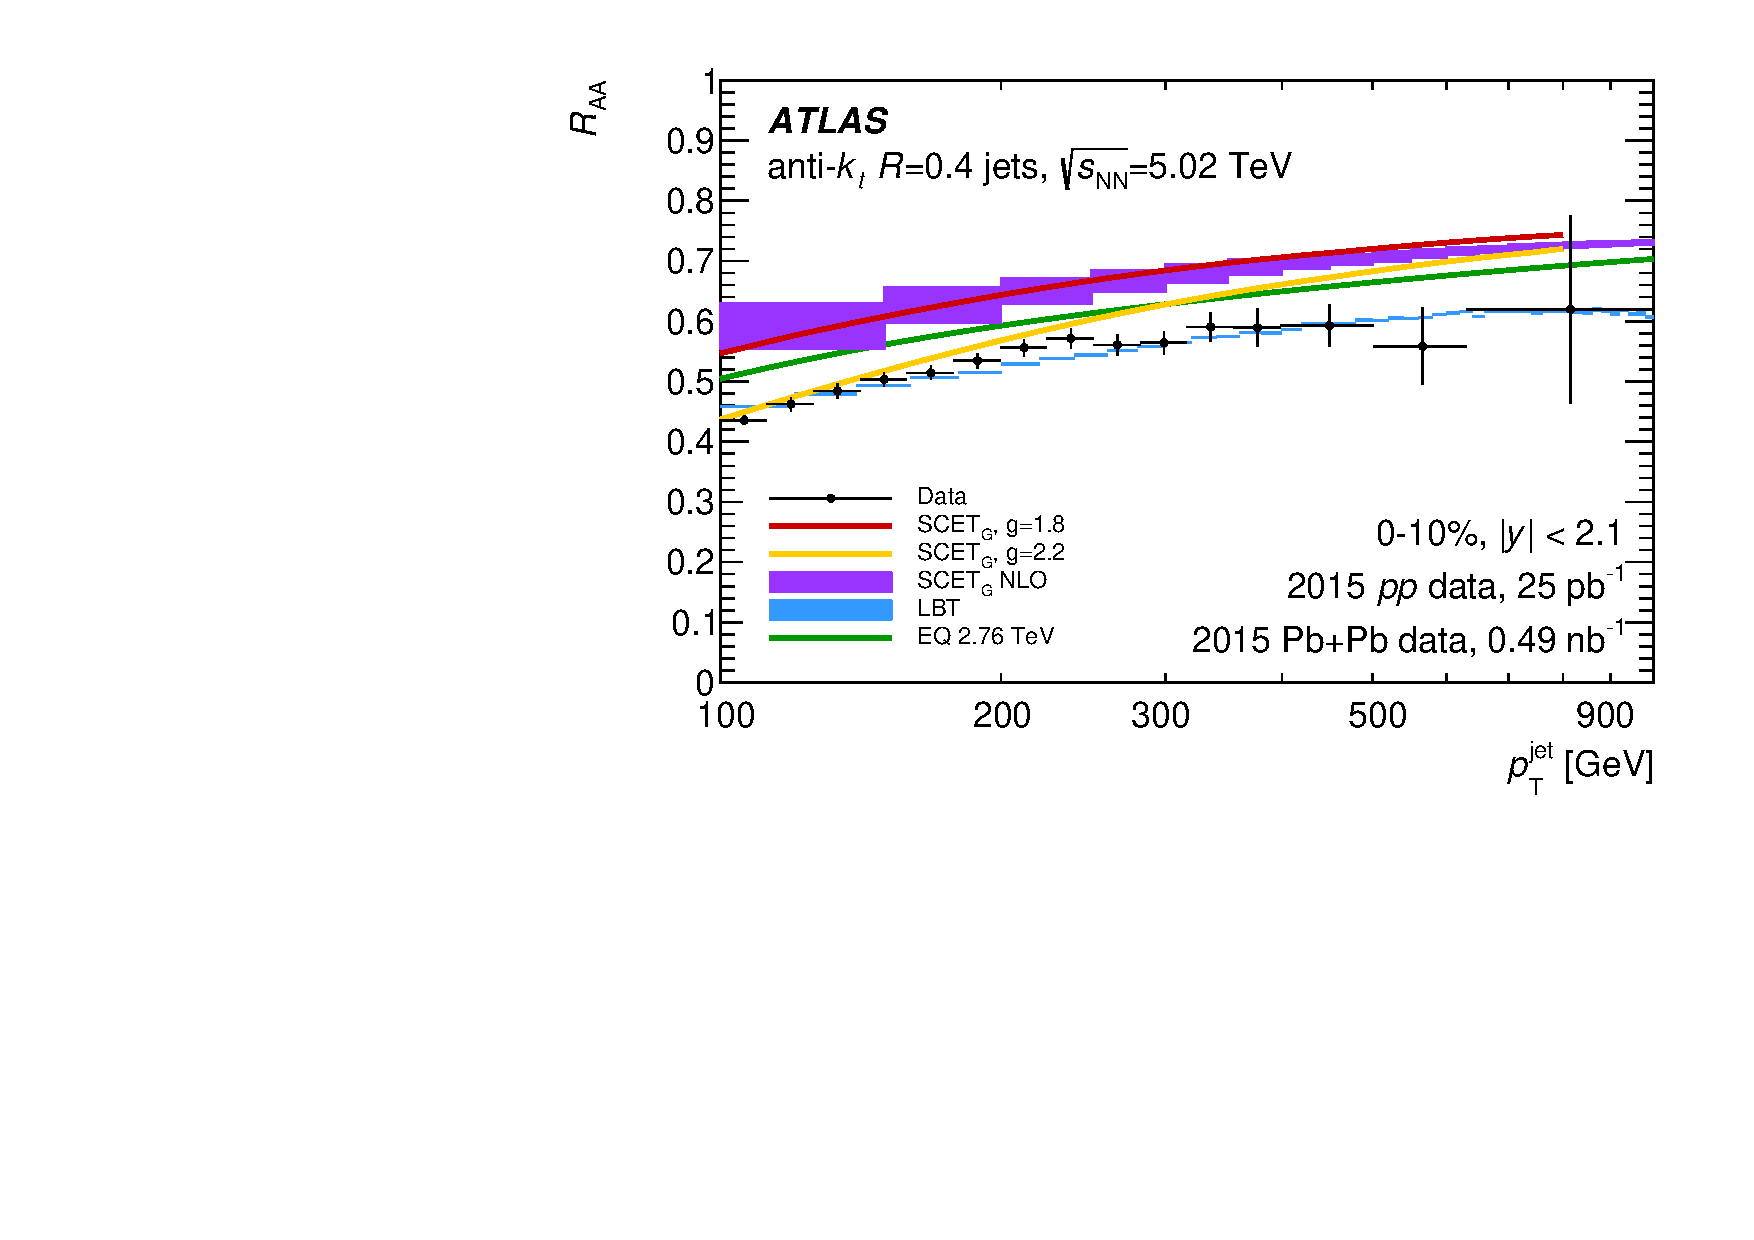
\includegraphics[width=0.65\textwidth]{fig/RAA_jet}\\
{\tiny  Figure is taken from {\color{teablue}
M.~Aaboud {\it et al.} [ATLAS Collaboration],
  %``Measurement of the nuclear modification factor for inclusive jets in Pb+Pb collisions at $\sqrt{s_\mathrm{NN}}=5.02$ TeV with the ATLAS detector,''
  Phys.\ Lett.\ B {\bf 790}, 108 (2019).
  }}
\end{center}
\vspace{2mm}
\begin{enumerate}
\item{\large There are many "good" models for jet quenching.}
\vspace{4mm}
\item{\large Differences can mostly trace back to the modelling of  bulk matter.}
\vspace{4mm}
\item{\large\bf\color{darkred} Let us take a top-down approach from QCD!}
\end{enumerate}
\end{frame}
%
%%%%%%%%%%%%%%%%%%%%%%%%%%%%%%%%%%%%%%%%%%%%%%%%%%%%%%%%%%
%
\begin{frame}{\bf\huge Everything starts from QCD on the SK contour.}	\vspace{2mm}
\begin{enumerate}
\item{\large Time-dependent observations are calculated in QFT on}
\vspace{2mm}
\begin{center}
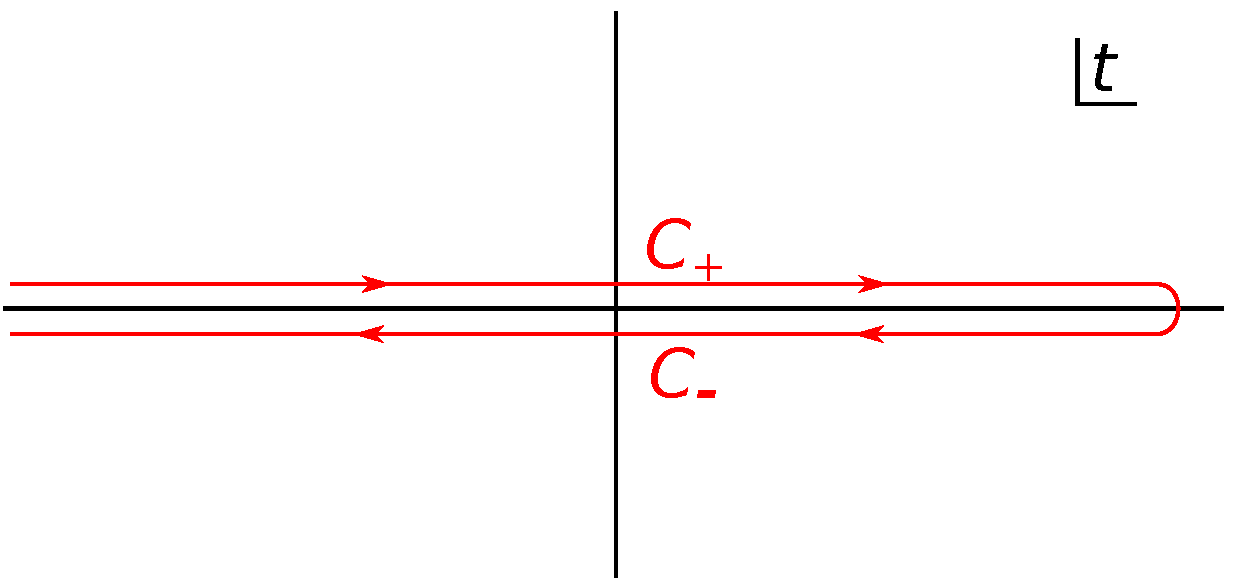
\includegraphics[width=0.65\textwidth]{fig/SKcontour}\\
{\tiny {\color{teablue}
Schwinger, {\emph{J.Math.Phys.} {\bfseries 2}
  (1961) 407--432}; Keldysh,
  {\emph{Zh.Eksp.Teor.Fiz.} {\bfseries 47} (1964) 1515--1527}.
  }}
\end{center}
\vspace{2mm}
\item{\large Equivalently, double the fields:}
\begin{align}
    \mathcal{L}_{QCD, I}(\phi)\to \mathcal{L}_{QCD, I}(\Phi_{+}) - \mathcal{L}_{QCD, I}(\Phi_{-})\notag
\end{align}
with $\Phi$ quark and gluon fields and $\Phi_\pm$ fields respectively on $C_\pm$.\\
\begin{center}
{\tiny For a recent discussion in QCD, see {\color{teablue}
 Jeon, {\emph{Annals Phys.}
  {\bfseries 340} (2014) 119--170};   BW and Kovchegov,
  %``Time-dependent observables in heavy ion collisions. Part I. Setting up the formalism,''
  JHEP {\bf 1803}, 158 (2018).
  }}
\end{center}
\end{enumerate}
\end{frame}

%
%%%%%%%%%%%%%%%%%%%%%%%%%%%%%%%%%%%%%%%%%%%%%%%%%%%%%%%%%%
%
\begin{frame}{\bf\huge Jet production}
\vspace{4mm}
\begin{center}
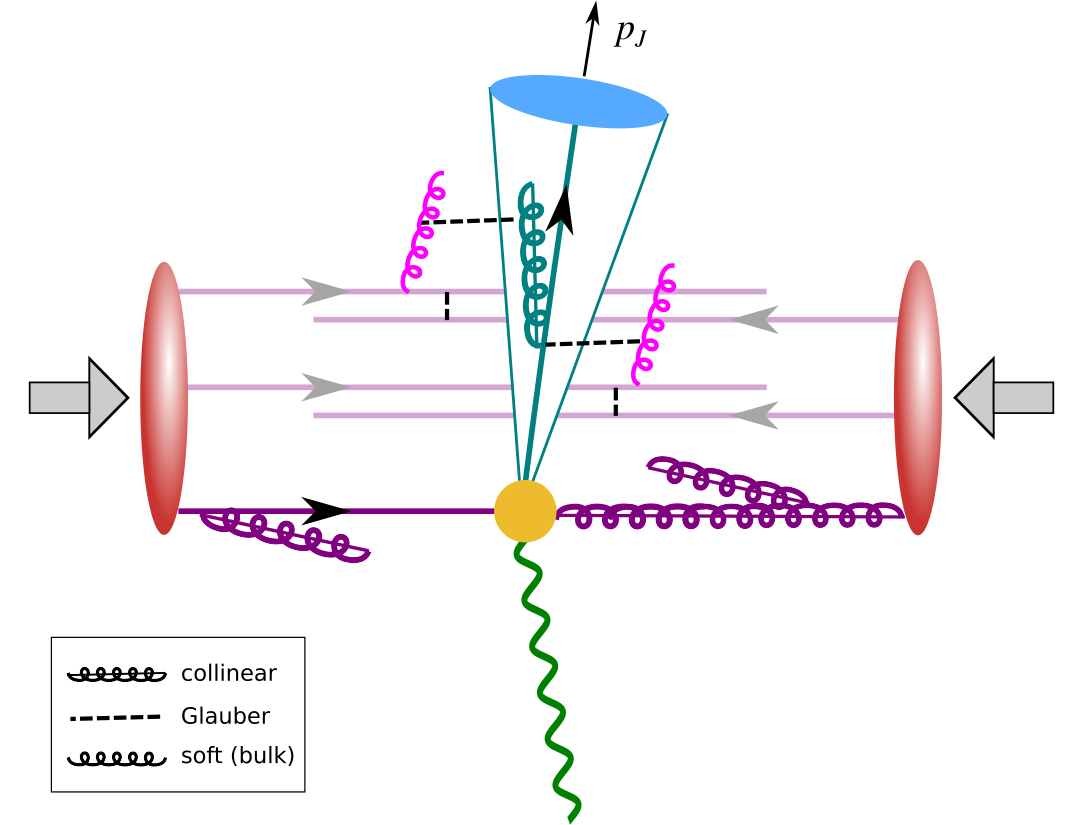
\includegraphics[width=0.6\textwidth]{fig/AA}\\
\end{center}
\vspace{2mm}
{\large In jet production, we measure:}
\begin{enumerate}
    \item{\large Jets}
    \item{\large Soft particles to determine centrality}
\end{enumerate}
\end{frame}
%
%%%%%%%%%%%%%%%%%%%%%%%%%%%%%%%%%%%%%%%%%%%%%%%%%%%%%%%%%%
%
\begin{frame}{\bf\huge Jet \& bulk: QCD Factorization}	\vspace{4mm}
\begin{center}
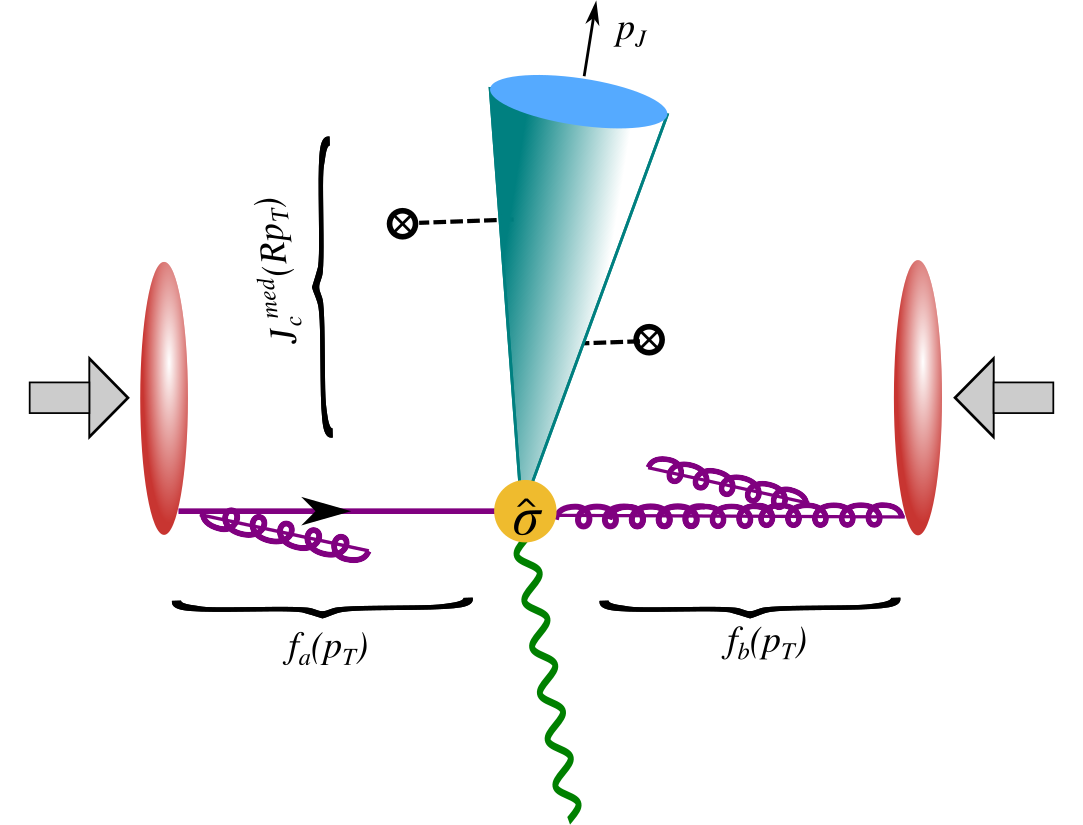
\includegraphics[width=0.6\textwidth]{fig/facotrization}\\
\end{center}
%\vspace{2mm}
\begin{enumerate}
\item{A factorization formula:}
\begin{align}
    \frac{d\sigma}{dp_{T} d\eta} =\sum\limits_{abc}f_a\otimes f_b \otimes \hat{\sigma}_{ab\to c}\otimes \underbrace{J_c^{med}}_{\text{\color{darkred}Bulk enters.}}\notag
\end{align}
\begin{center}
{\tiny  For a recent discussion: {\color{teablue}
  Qiu, Ringer, Sato and Zurita,
  %``Factorization of jet cross sections in heavy-ion collisions,''
  Phys.\ Rev.\ Lett.\  {\bf 122}, no. 25, 252301 (2019)
  %[arXiv:1903.01993 [hep-ph]]
  .
  }}\\
  \vspace{2mm}
 {\color{darkred}\bf A better understanding of bulk is need!
 %$\textcircled{1}$ a proof in QCD is still missing!
 }
\end{center}
\end{enumerate}
\end{frame}
%
%%%%%%%%%%%%%%%%%%%%%%%%%%%%%%%%%%%%%%%%%%%%%%%%%%%%%%%%%%
%
\begin{frame}{\bf\huge The Bjorken Picture}	\vspace{4mm}
\begin{center}
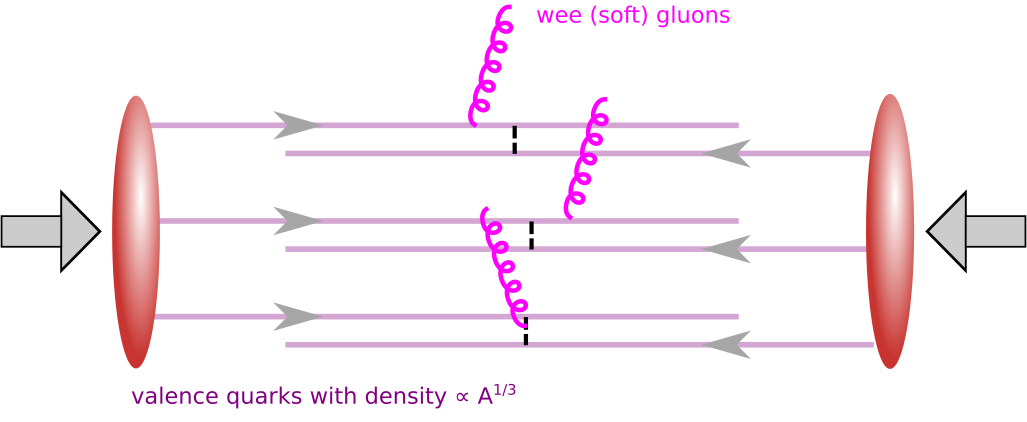
\includegraphics[width=0.65\textwidth]{fig/Bjorken}\\
{\tiny  {\color{teablue}
Bjorken,
  %``Hadron Final States in Deep Inelastic Processes,''
  Lect.\ Notes Phys.\  {\bf 56}, 93 (1976).
  }}
\end{center}
%\vspace{4mm}
% {\large How far one can go beyond such a parton picture?}
\begin{enumerate}
\item{\large The valence quarks pass through each other.}
\vspace{2mm}
\item{\large Soft ("wee") partons are freed from the wave function.}
\vspace{2mm}
\item{\large Product: a central plateau in the rapidity distribution.}\\
\vspace{1mm}
    longitudinal boost invariance (around mid-rapidity)
\vspace{1mm}
\item{\large The modern revival: the saturation model (CGC)}
\begin{center}
    {\tiny  A comprehensive review: {\color{teablue}
  Kovchegov and Levin,
  %``Quantum chromodynamics at high energy,''
  Camb.\ Monogr.\ Part.\ Phys.\ Nucl.\ Phys.\ Cosmol.\  {\bf 33}, 1 (2012).
  %%CITATION = doi:10.1017/CBO9781139022187;%%
  %178 citations counted in INSPIRE as of 25 May 2020
.
  }}
\end{center}
\end{enumerate}
\vspace{1mm}
\begin{center}
{\bf\large A complete understanding starting from this parton picture?}
\end{center}

\end{frame}
%
%%%%%%%%%%%%%%%%%%%%%%%%%%%%%%%%%%%%%%%%%%%%%%%%%%%%%%%%%%
%
\begin{frame}{\bf\huge The lowest order calculation on $C_\pm$}	\vspace{2mm}
\begin{align}
\text{\tiny $G_{22}^{a\mu,b\nu}(X, p)$}=\begin{array}{c}
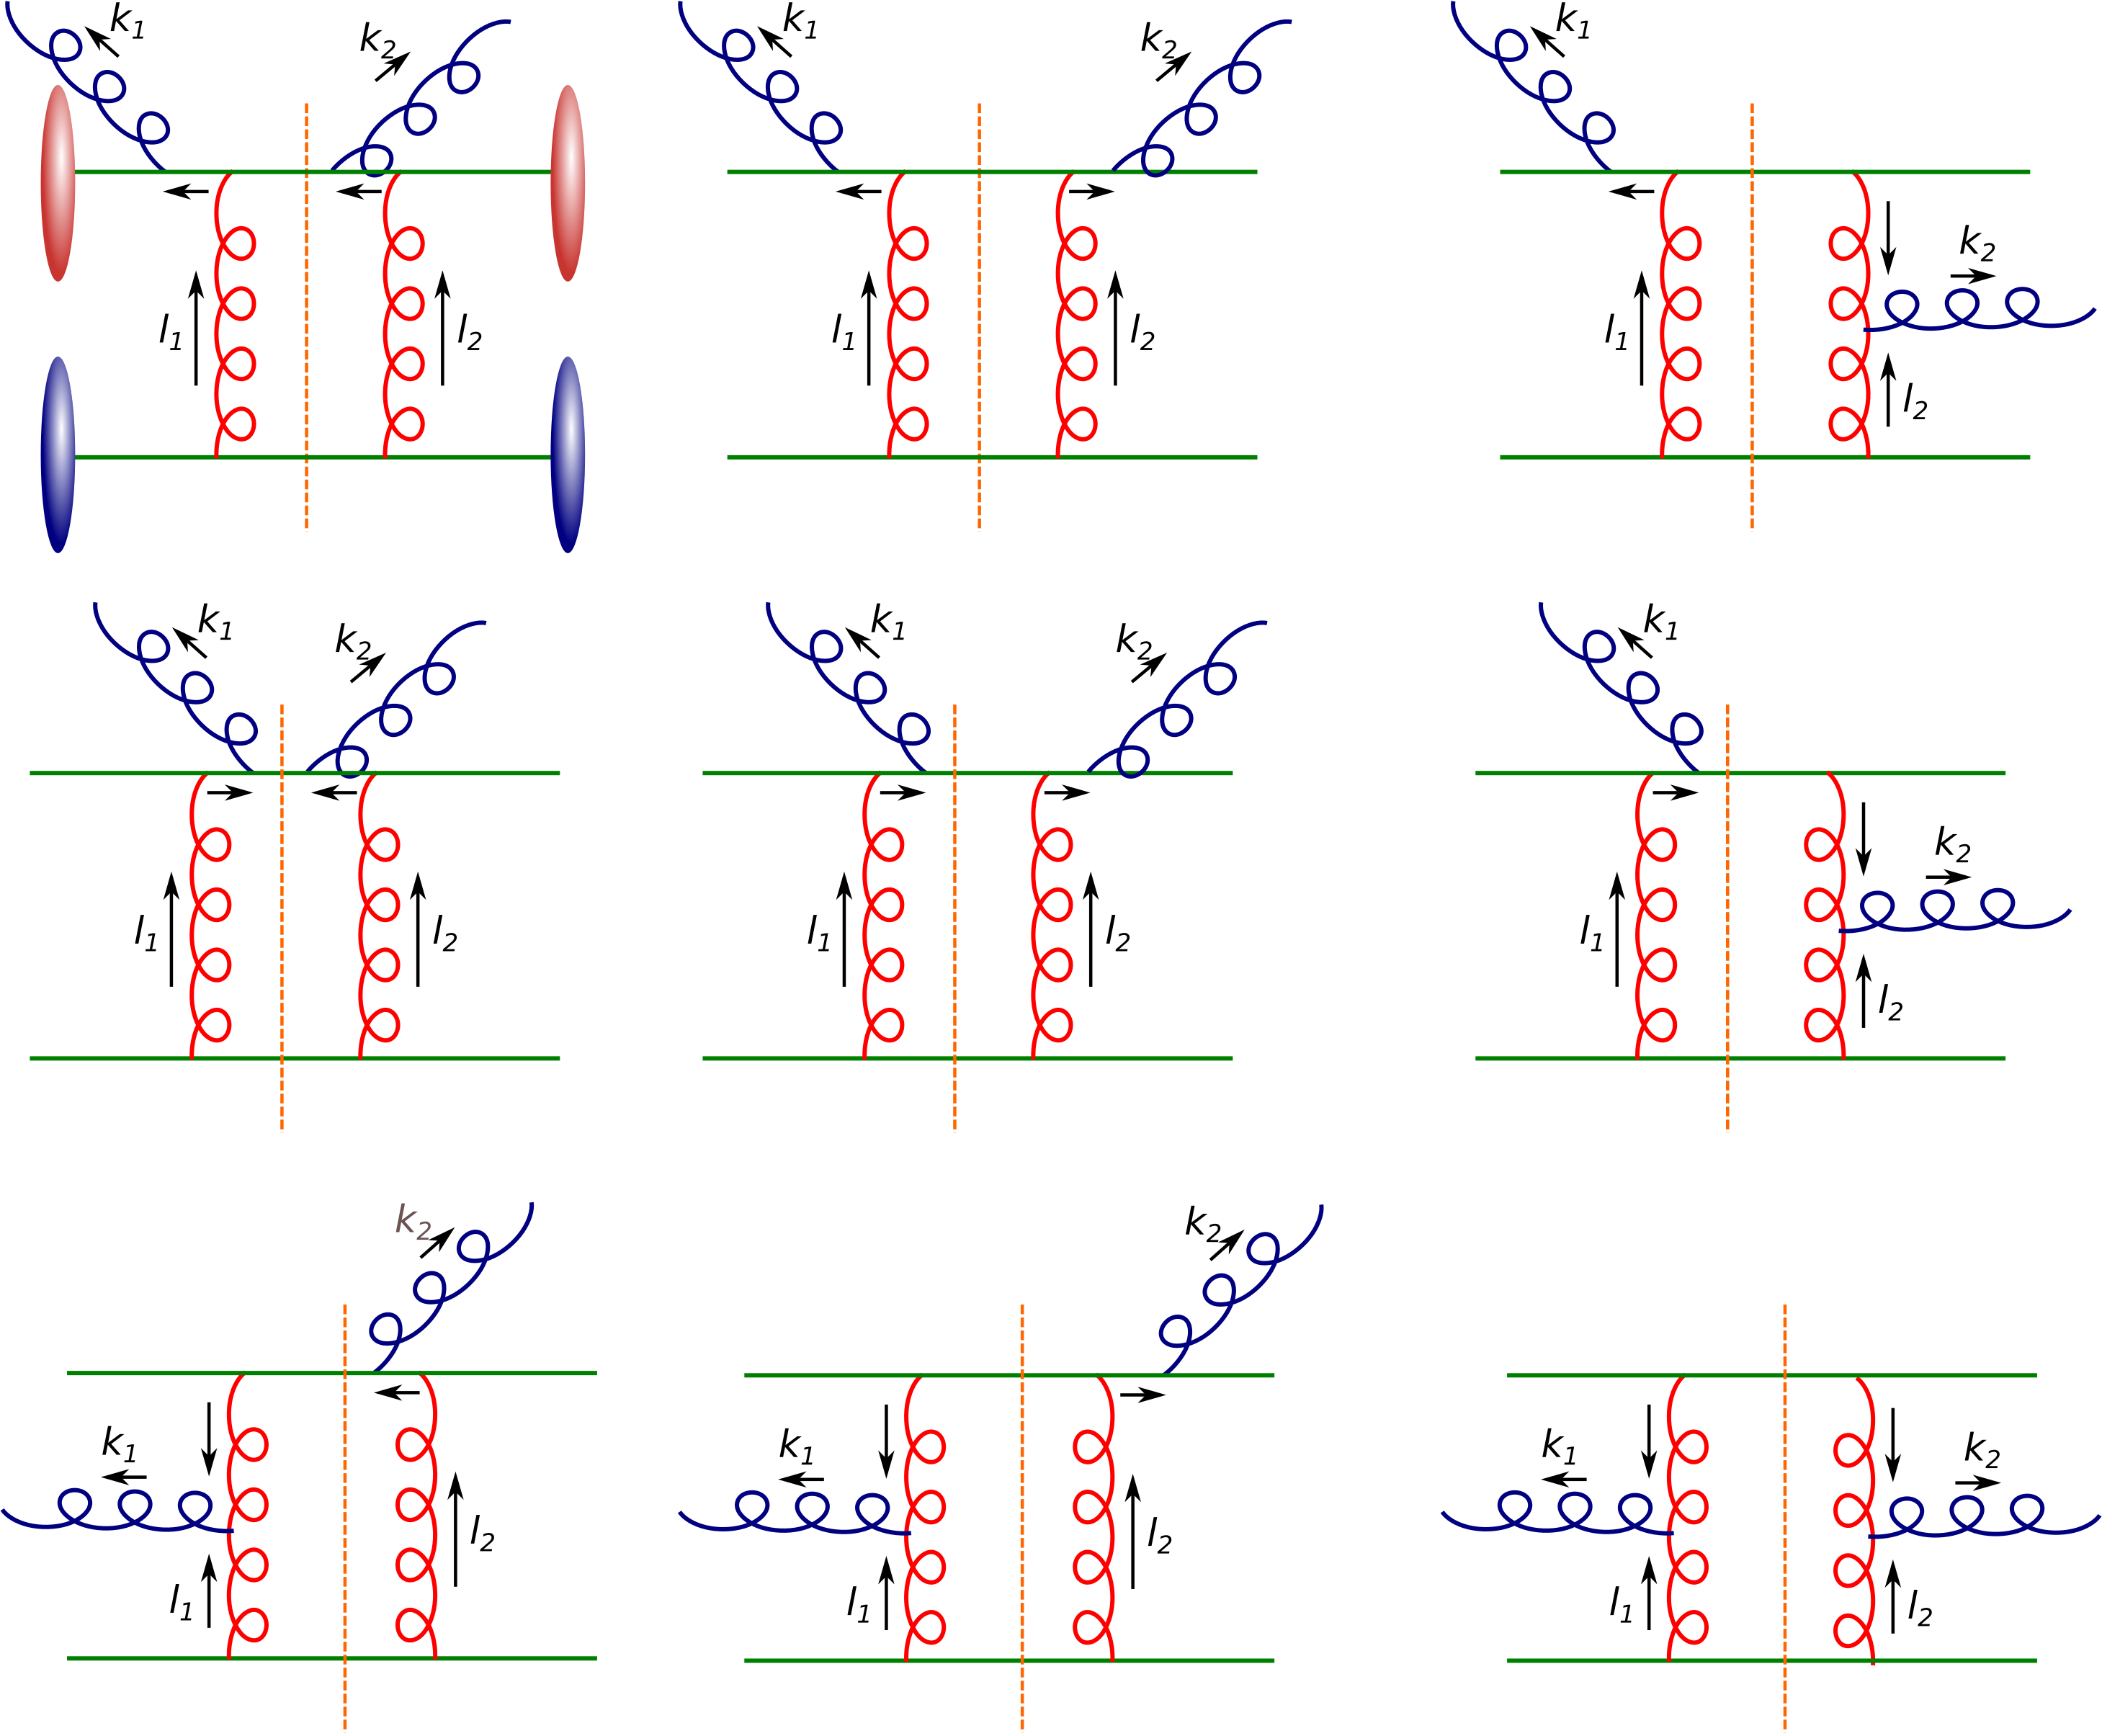
\includegraphics[width=0.45\textwidth]{fig/G22NLO}
\end{array}\text{\tiny $\to  2\pi\delta(p^2) \delta^{ab}
  \sum\limits_{\lambda=\pm}\epsilon_\lambda^\mu(p)
  \epsilon_{\lambda}^{*\nu}(p) f^{cl}(X,p)$}\notag
\end{align}
{\large\bf At $O(\alpha_s A^{2/3})$ and large $\tau$}
\begin{align}
  f^{cl}(X,p)=\frac{1}{\tau} \theta(X^+) \theta(X^-) \delta(y-\eta)
  f_\perp^{cl}(\underline{p})
  \notag
\end{align}
with $y = \frac{1}{2}\ln\frac{p^+}{p^-}$, $\eta = \frac{1}{2}\ln\frac{X^+}{X^-}$ and
$f_\perp^{cl}(\underline{p})\equiv\frac{8\pi^2\alpha_s^3}{N_c}\left(\frac{A}{S_\perp}\right)^2
  \frac{1}{p_T^5}\ln\left(\frac{p_T^2}{\Lambda^2}\right).$
  \vspace{1mm}
\begin{center}
    {\tiny  {\color{teablue}
  BW and Kovchegov,
  %``Time-dependent observables in heavy ion collisions. Part I. Setting up the formalism,''
  JHEP {\bf 1803}, 158 (2018)
  [arXiv:1709.02866 [hep-ph]].
}}
\end{center}
% \vspace{2mm}
% \item{\large \color{darkred}\bf The Bjorken or Landau pictures?}
% \vspace{2mm}
% \begin{center}
% 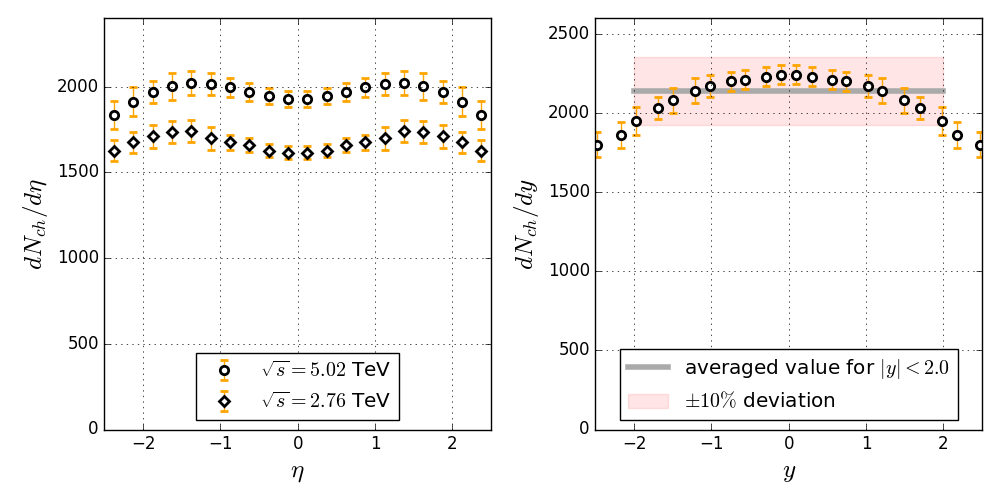
\includegraphics[width=0.65\textwidth]{fig/multiplicity}\\
%     {\tiny {\color{teablue}
% ALICE Collaboration:
%   %``Centrality dependence of the pseudorapidity density distribution for charged particles in Pb-Pb collisions at $\sqrt{s_{\rm NN}}=5.02$ TeV,''
%   Phys.\ Lett.\ B {\bf 726}, 610 (2013); Phys.\ Lett.\ B {\bf 772}, 567 (2017).
% }}
% \end{center}

%\end{enumerate}
\end{frame}
% %
% %%%%%%%%%%%%%%%%%%%%%%%%%%%%%%%%%%%%%%%%%%%%%%%%%%%%%%%%%%
% %
% \setcounter{page}{0}
% \begin{frame}
% \topskip0pt
% \vspace*{\fill}
% \begin{center}
% {\Huge\bf\color{gray} Tools in our toolbox}
% \end{center}
% \vspace*{\fill}
% \end{frame}
% %
% %%%%%%%%%%%%%%%%%%%%%%%%%%%%%%%%%%%%%%%%%%%%%%%%%%%%%%%%%%
% %
% \begin{frame}{\bf\huge The Color-Glass Condensate}	\vspace{4mm}
% \begin{center}
% 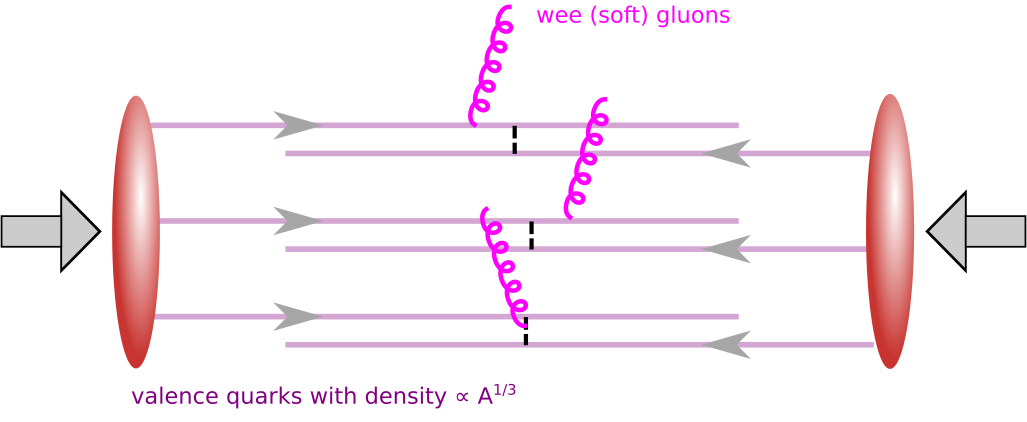
\includegraphics[width=0.65\textwidth]{fig/Bjorken}\\
% {\tiny  {\color{teablue}
% Bjorken,
%   %``Hadron Final States in Deep Inelastic Processes,''
%   Lect.\ Notes Phys.\  {\bf 56}, 93 (1976).
%   }}
% \end{center}
% %\vspace{4mm}
% \begin{enumerate}
% \item{The modern revivial: saturation physics (color-glass condensate)}\\
% \begin{center}
%     {\tiny  {\color{teablue}
%   Kovchegov and Levin,
%   %``Quantum chromodynamics at high energy,''
%   Camb.\ Monogr.\ Part.\ Phys.\ Nucl.\ Phys.\ Cosmol.\  {\bf 33}, 1 (2012).
%   %%CITATION = doi:10.1017/CBO9781139022187;%%
%   %178 citations counted in INSPIRE as of 25 May 2020
% .
%   }}
% \end{center}
% \item{The longitudinal boost-invariance:}\\
% \vspace{1mm}
% {\small For example, at $O(\alpha_s A^{2/3})$ and large $\tau$}
% \begin{align}
%   f^{cl}(X,p)=\frac{1}{\tau} \theta(X^+) \theta(X^-) \delta(y-\eta)
%   f_\perp^{cl}(\underline{p})
%   \notag
% \end{align}
% with
% $f_\perp^{cl}(\underline{p})\equiv\frac{8\pi^2\alpha_s^3}{N_c}\left(\frac{A}{S_\perp}\right)^2
%   \frac{1}{p_T^5}\ln\left(\frac{p_T^2}{\Lambda^2}\right).$
% \begin{center}
%     {\tiny  {\color{teablue}
% \bibitem{Wu:2017rry} 
%   BW and Kovchegov,
%   %``Time-dependent observables in heavy ion collisions. Part I. Setting up the formalism,''
%   JHEP {\bf 1803}, 158 (2018)
%   [arXiv:1709.02866 [hep-ph]].
% }}
% \end{center}
% \end{enumerate}
% \end{frame}
%
%%%%%%%%%%%%%%%%%%%%%%%%%%%%%%%%%%%%%%%%%%%%%%%%%%%%%%%%%%
%https://www.overleaf.com/project/5ec7eb5acba0510001502bd9
\setcounter{page}{0}
\begin{frame}
\topskip0pt
\vspace*{\fill}
\begin{center}
{\Huge\bf\color{gray} Bulk in AA collisions}
\end{center}
\vspace*{\fill}
\end{frame}
%
%%%%%%%%%%%%%%%%%%%%%%%%%%%%%%%%%%%%%%%%%%%%%%%%%%%%%%%%%%
%
\setcounter{page}{7}
\begin{frame}{\bf\huge The Bottom-up Thermalization}	\vspace{2mm}
\begin{center}
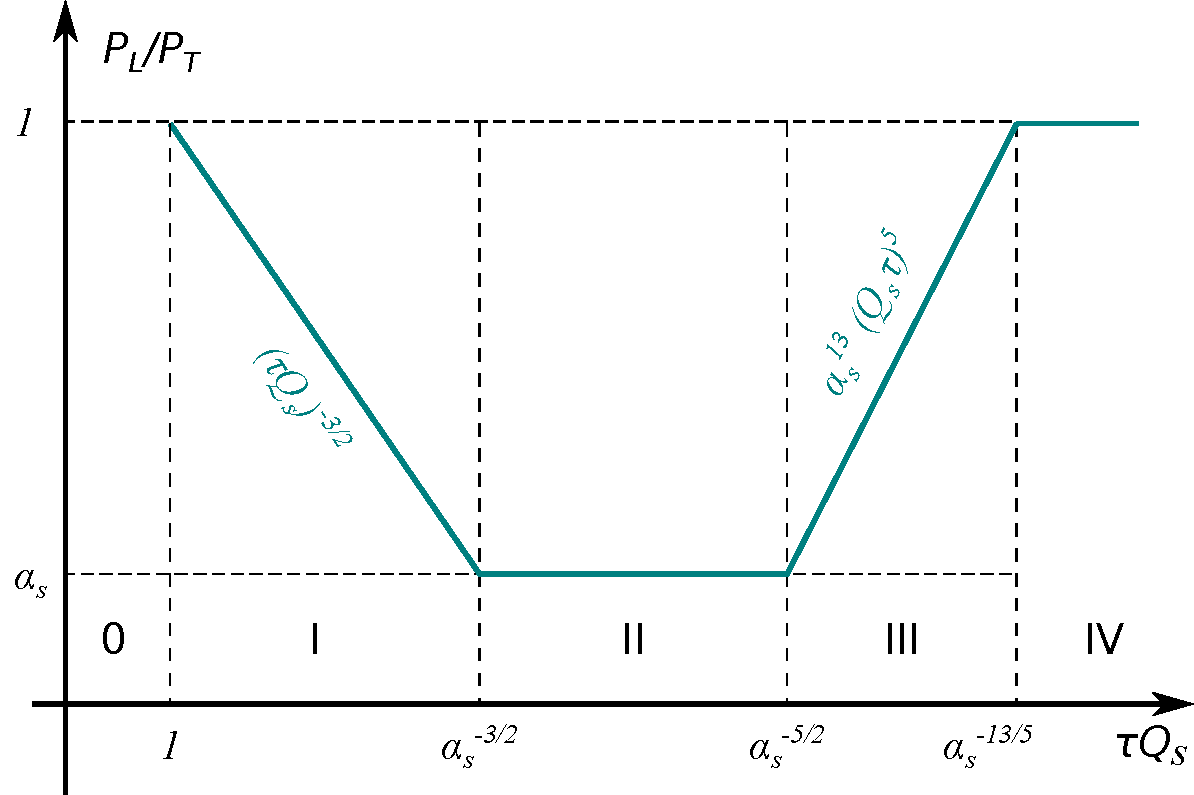
\includegraphics[width=0.6\textwidth]{fig/PLoPT}\\
\vspace{4mm}
% \begin{tabular}{ c|| c c c c c c}
% \hline
% time interval& hard $f$ & soft $f$&$\frac{N_h}{Q_s^3}$ & $\frac{N_s}{Q_s^3}$ & $\frac{\epsilon}{Q_s^4}$ & $\frac{P_L}{P_T}$\\
% \hline\hline
%  $ \alpha_s^{-\frac{3}{2}}> \tau Q_s > 1$ &$\frac{1}{\alpha_{s} (\tau Q_s)^{\frac{2}{3}}}$ & $\frac{1}{\alpha_{s} (\tau Q_s)^{\frac{1}{3}}}$ & $\frac{1}{\alpha_s \tau Q_s}$ & $\frac{1}{\alpha_s (\tau Q_s)^{\frac{4}{3}}}$ & $\frac{1}{\alpha_s \tau Q_s}$ & $\frac{1}{(\tau Q_s)^{\frac{2}{3}}}$\\
%  \hline
%  $ \alpha_s^{-\frac{5}{2}}> \tau Q_s > \alpha_s^{-\frac{3}{2}}$ &$\frac{1}{\alpha_{s}^{\frac{3}{2}} \tau Q_{s} }$ & $\frac{1}{\alpha_{s}^{\frac{5}{4}} (\tau Q_s)^{\frac{1}{2}}}$ & $\frac{1}{\alpha_s \tau Q_s}$ & $\frac{ \alpha_{s}^{\frac{1}{4}}}{(\tau Q_s)^{\frac{1}{2}}}\right]$$ & $\frac{1}{\alpha_s \tau Q_s}$ & $\alpha_s$\\
%   \hline
%  $ \alpha_s^{-\frac{13}{5}}> \tau Q_s > \alpha_s^{-\frac{5}{2}}$ &$\frac{1}{\alpha_{s} (\tau Q_s)^{\frac{2}{3}}}$ & $\frac{1}{\alpha_{s} (\tau Q_s)^{\frac{1}{3}}}$ & $\frac{1}{\alpha_s \tau Q_s}$ & $\frac{1}{\alpha_s (\tau Q_s)^{\frac{4}{3}}}$ & $\frac{1}{\alpha_s \tau Q_s}$ & $ \alpha_{s}^{13} (\tau Q_s)^{5}$\\
%  %$ \alpha_s^{-\frac{5}{2}}> \tau Q_s > \alpha_s^{-\frac{3}{2}}$ & cell5 & cell6 \\  
%  %cell7 & cell8 & cell9    
%  \hline
% \end{tabular}\\
\begin{tabular}{ c|| c c c c c c}
\hline
time interval&$N_s/N_h$ & $\epsilon_s/Q_s^4$ & $\tau/\tau_{th}$ & $T$\\
\hline\hline
 $ \alpha_s^{-\frac{3}{2}}> \tau Q_s > 1$ 
 & $(\tau Q_s)^{-\frac{1}{3}}$ 
 & $\alpha_{s}^{-1} (\tau Q_s)^{-\frac{5}{3}}$
 & $\alpha_{s}^{\frac{7}{4}} (\tau Q_s)^{\frac{7}{12}}$
 &0\\
 \hline
 $ \alpha_s^{-\frac{5}{2}}> \tau Q_s > \alpha_s^{-\frac{3}{2}}$ 
 & $\alpha_{s}^{\frac{5}{4}} (\tau Q_s)^{\frac{1}{2}}$
 & $\alpha_{s}^{\frac{3}{4}}(\tau Q_s)^{-\frac{1}{2}}$
 & $\alpha_{s}^{\frac{35}{16}} (\tau Q_s)^{\frac{7}{8}}$
 &0\\
  \hline
 $ \alpha_s^{-\frac{13}{5}}> \tau Q_s > \alpha_s^{-\frac{5}{2}}$ 
 & $\alpha_{s}^{10} (\tau Q_s)^{4}$
 & $\alpha_{s}^{12} (\tau Q_s)^{4}$ 
 & $ \alpha_{s}^{5} (\tau Q_s)^{2}$
 & $ \alpha_{s}^{3} Q_{s}^{2} \tau$\\
 %$ \alpha_s^{-\frac{5}{2}}> \tau Q_s > \alpha_s^{-\frac{3}{2}}$ & cell5 & cell6 \\  
 %cell7 & cell8 & cell9    
 \hline
\end{tabular}\\
\vspace{2mm}
{\small Note that $N_h \sim Q_s^2/(\alpha_s\tau)$ and $\epsilon_h\sim Q_s N_h$.}\\
\vspace{2mm}
    {\tiny  {\color{teablue}
  Baier, Mueller, Schiff and Son,
  %``'Bottom up' thermalization in heavy ion collisions,''
  Phys.\ Lett.\ B {\bf 502}, 51 (2001)
  [hep-ph/0009237].
}}
\end{center}
\end{frame}
%
%%%%%%%%%%%%%%%%%%%%%%%%%%%%%%%%%%%%%%%%%%%%%%%%%%%%%%%%%%
%
\begin{frame}{\bf\huge The Bottom-up Thermalization}	\vspace{2mm}
{\large\bf Implication for jet quenching:}
\vspace{2mm}
\begin{center}
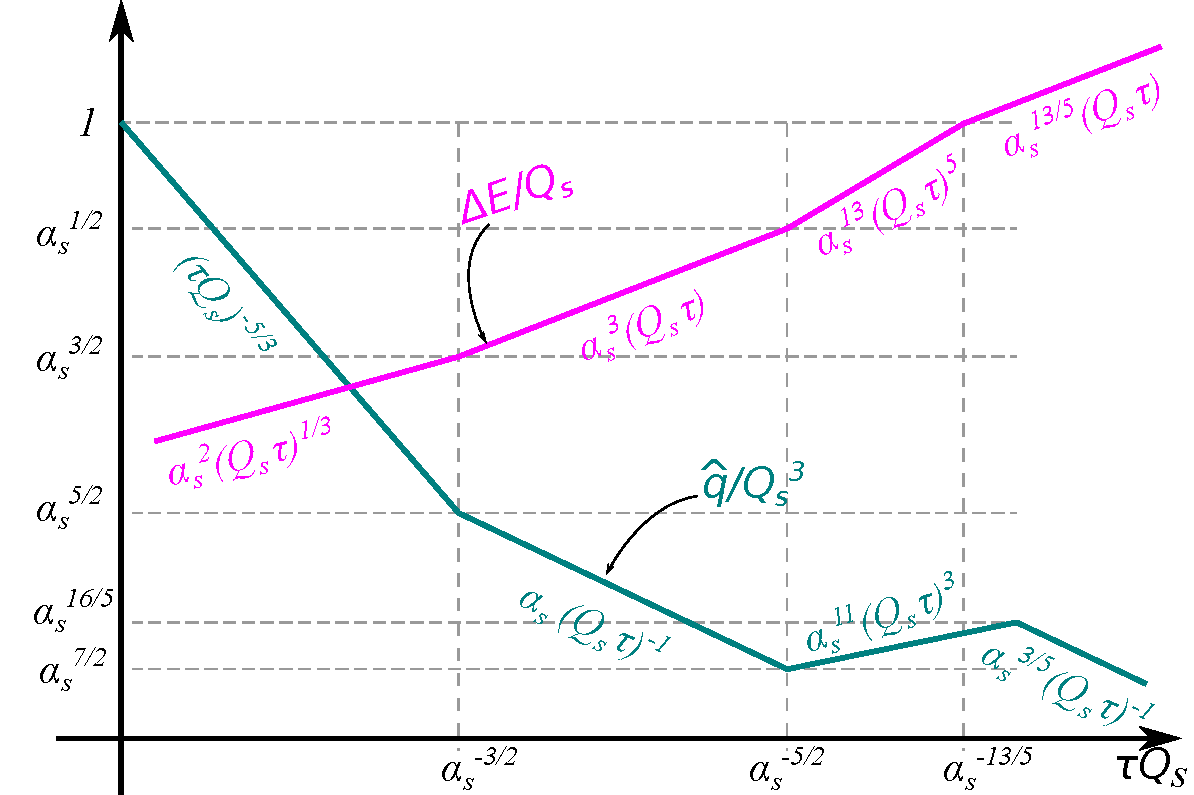
\includegraphics[width=0.8\textwidth]{fig/qhatInBottomUp}\end{center}
\end{frame}
%
%%%%%%%%%%%%%%%%%%%%%%%%%%%%%%%%%%%%%%%%%%%%%%%%%%%%%%%%%%
%
\begin{frame}{\bf\huge Some detailed calculation}	\vspace{2mm}
{\large\bf Detail calculations:}
\vspace{2mm}
\begin{enumerate}
    \item 
    \item
    \item
\end{enumerate}
\end{frame}
%
%%%%%%%%%%%%%%%%%%%%%%%%%%%%%%%%%%%%%%%%%%%%%%%%%%%%%%%%%%
%
\begin{frame}{\bf\huge Focus: Probing the Inner Workings of QGP}	\vspace{4mm}
\setcounter{page}{1}
\begin{center}
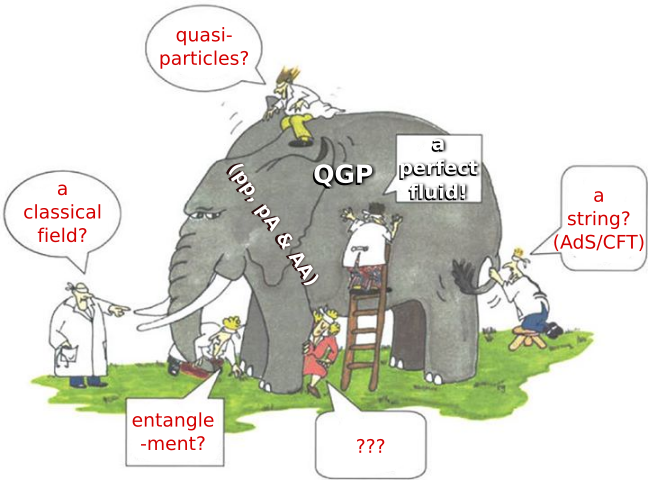
\includegraphics[width=0.65\textwidth]{fig/beyondhydro}
\vspace{4mm}
\begin{enumerate}
\item {Hydro has been very phenomenologically successful.}
\vspace{4mm}
\item {\color{darkred} Studying the inner workings of QGP now lies beyond hydro.}
\end{enumerate}
\end{center}
\end{frame}

%
%%%%%%%%%%%%%%%%%%%%%%%%%%%%%%%%%%%%%%%%%%%%%%%%%%%%%%%%%%
%
\setcounter{page}{5}
\begin{frame}{\bf\huge The Bottom-Up Thermalization}	\vspace{4mm}
\begin{center}
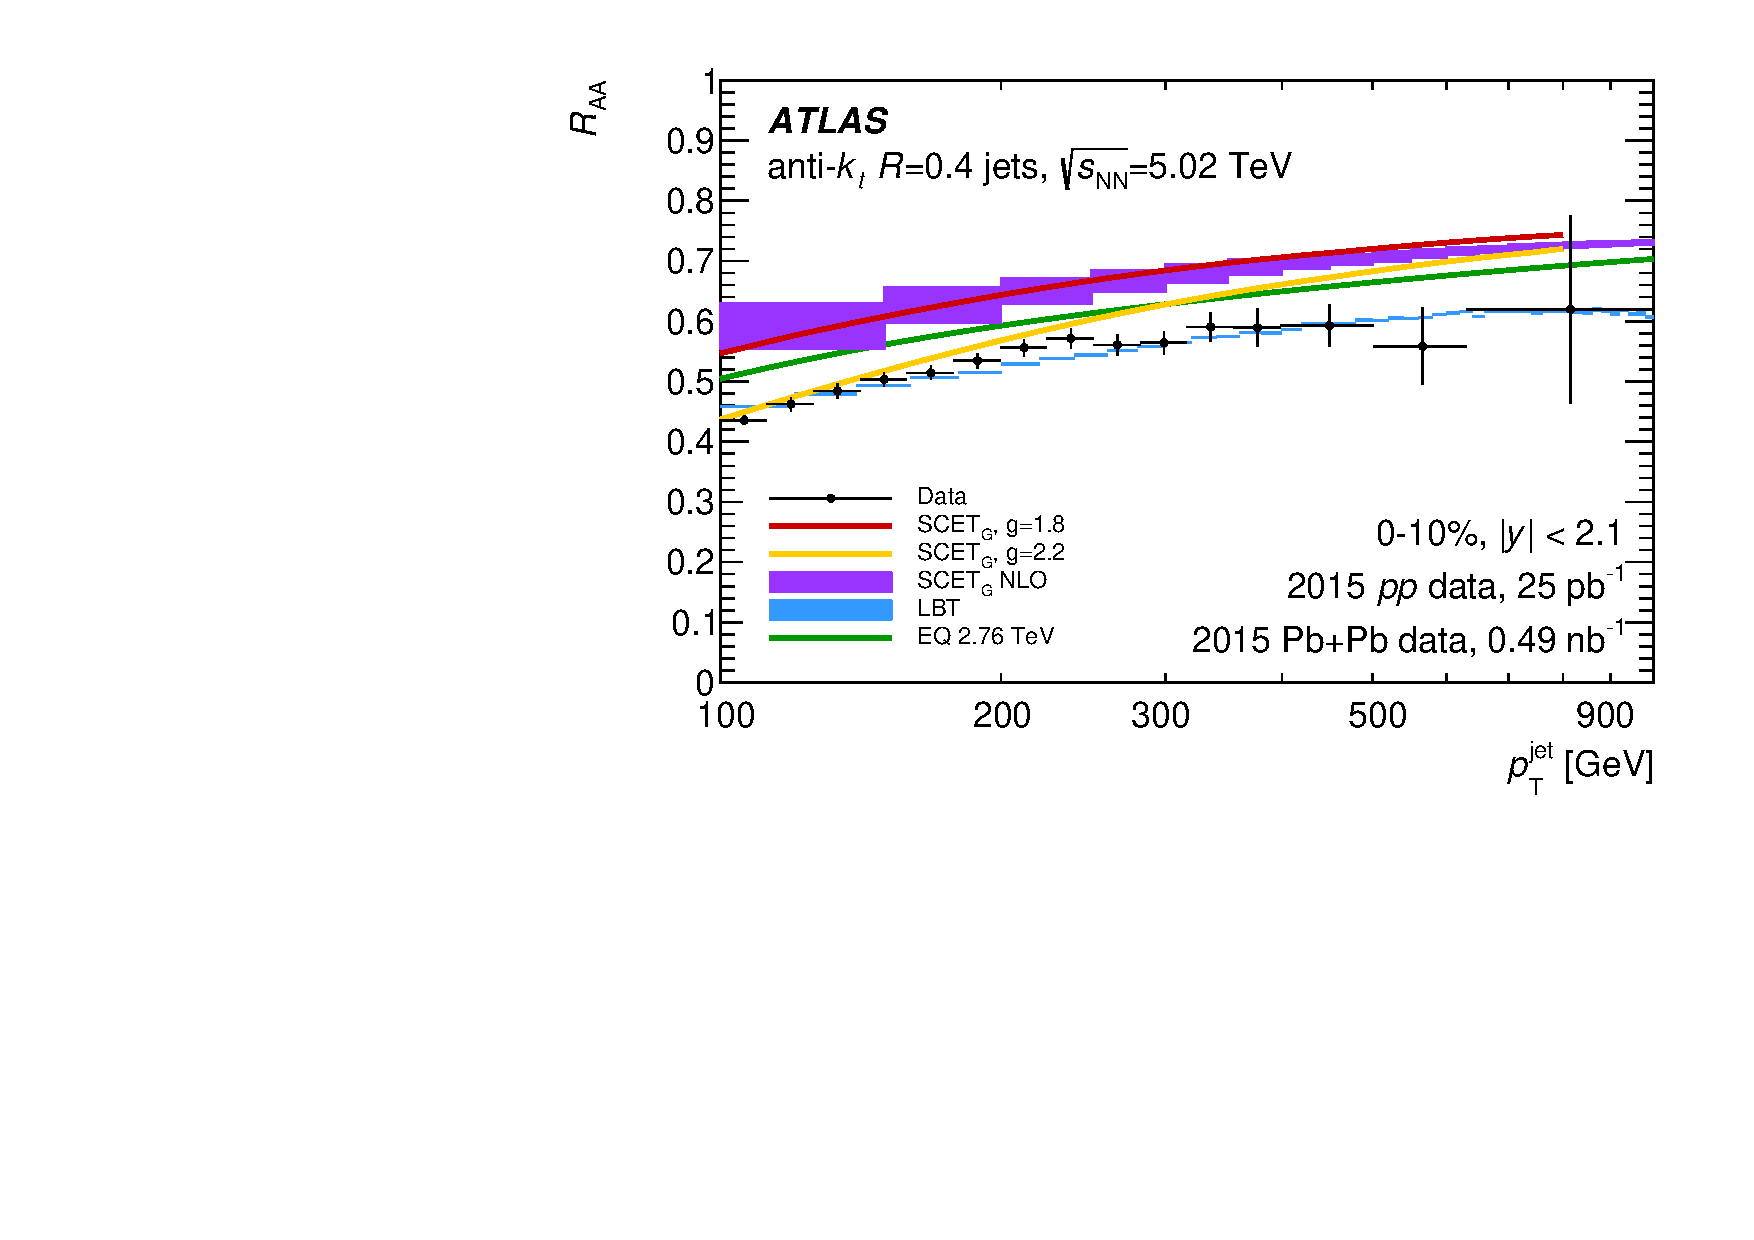
\includegraphics[width=0.65\textwidth]{fig/RAA_jet}\\
{\tiny  Figure is taken from {\color{teablue}
M.~Aaboud {\it et al.} [ATLAS Collaboration],
  %``Measurement of the nuclear modification factor for inclusive jets in Pb+Pb collisions at $\sqrt{s_\mathrm{NN}}=5.02$ TeV with the ATLAS detector,''
  Phys.\ Lett.\ B {\bf 790}, 108 (2019).
  }}
\end{center}
\vspace{4mm}
{\large It is broken:}
\vspace{2mm}
\begin{enumerate}
\item{small-$x$ evolution in QCD;}
\vspace{4mm}
\item{AdS/CFT.}
\end{enumerate}
\end{frame}

%
%%%%%%%%%%%%%%%%%%%%%%%%%%%%%%%%%%%%%%%%%%%%%%%%%%%%%%%%%%
%
\begin{frame}{\bf\huge The Medium-Induced Parton Energy Loss}	\vspace{4mm}
\begin{center}
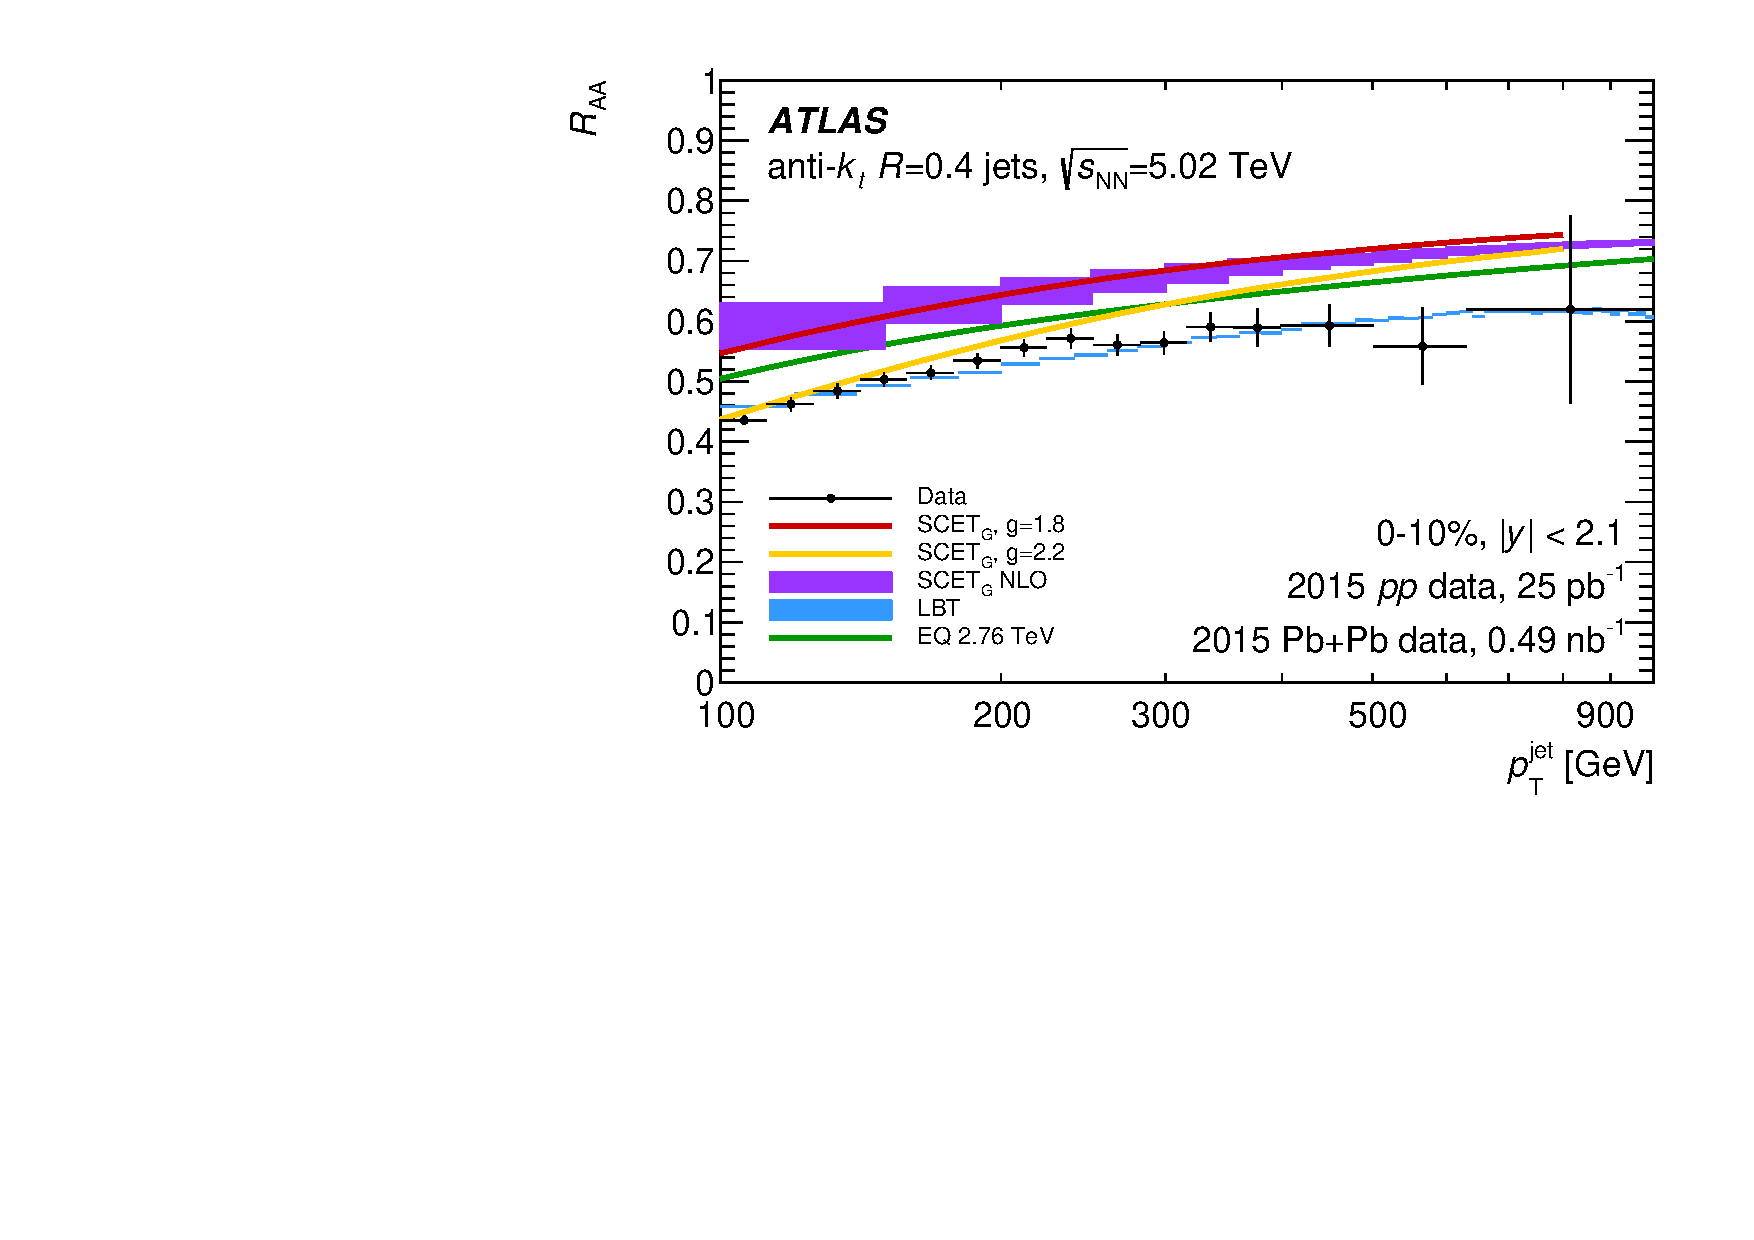
\includegraphics[width=0.65\textwidth]{fig/RAA_jet}\\
{\tiny  Figure is taken from {\color{teablue}
M.~Aaboud {\it et al.} [ATLAS Collaboration],
  %``Measurement of the nuclear modification factor for inclusive jets in Pb+Pb collisions at $\sqrt{s_\mathrm{NN}}=5.02$ TeV with the ATLAS detector,''
  Phys.\ Lett.\ B {\bf 790}, 108 (2019).
  }}
\end{center}
\vspace{4mm}
{\large It is broken:}
\vspace{2mm}
\begin{enumerate}
\item{small-$x$ evolution in QCD;}
\vspace{4mm}
\item{AdS/CFT.}
\end{enumerate}
\end{frame}
%
%%%%%%%%%%%%%%%%%%%%%%%%%%%%%%%%%%%%%%%%%%%%%%%%%%%%%%%%%%
%
\begin{frame}{\bf\huge High-Order Results}	\vspace{4mm}
\begin{center}
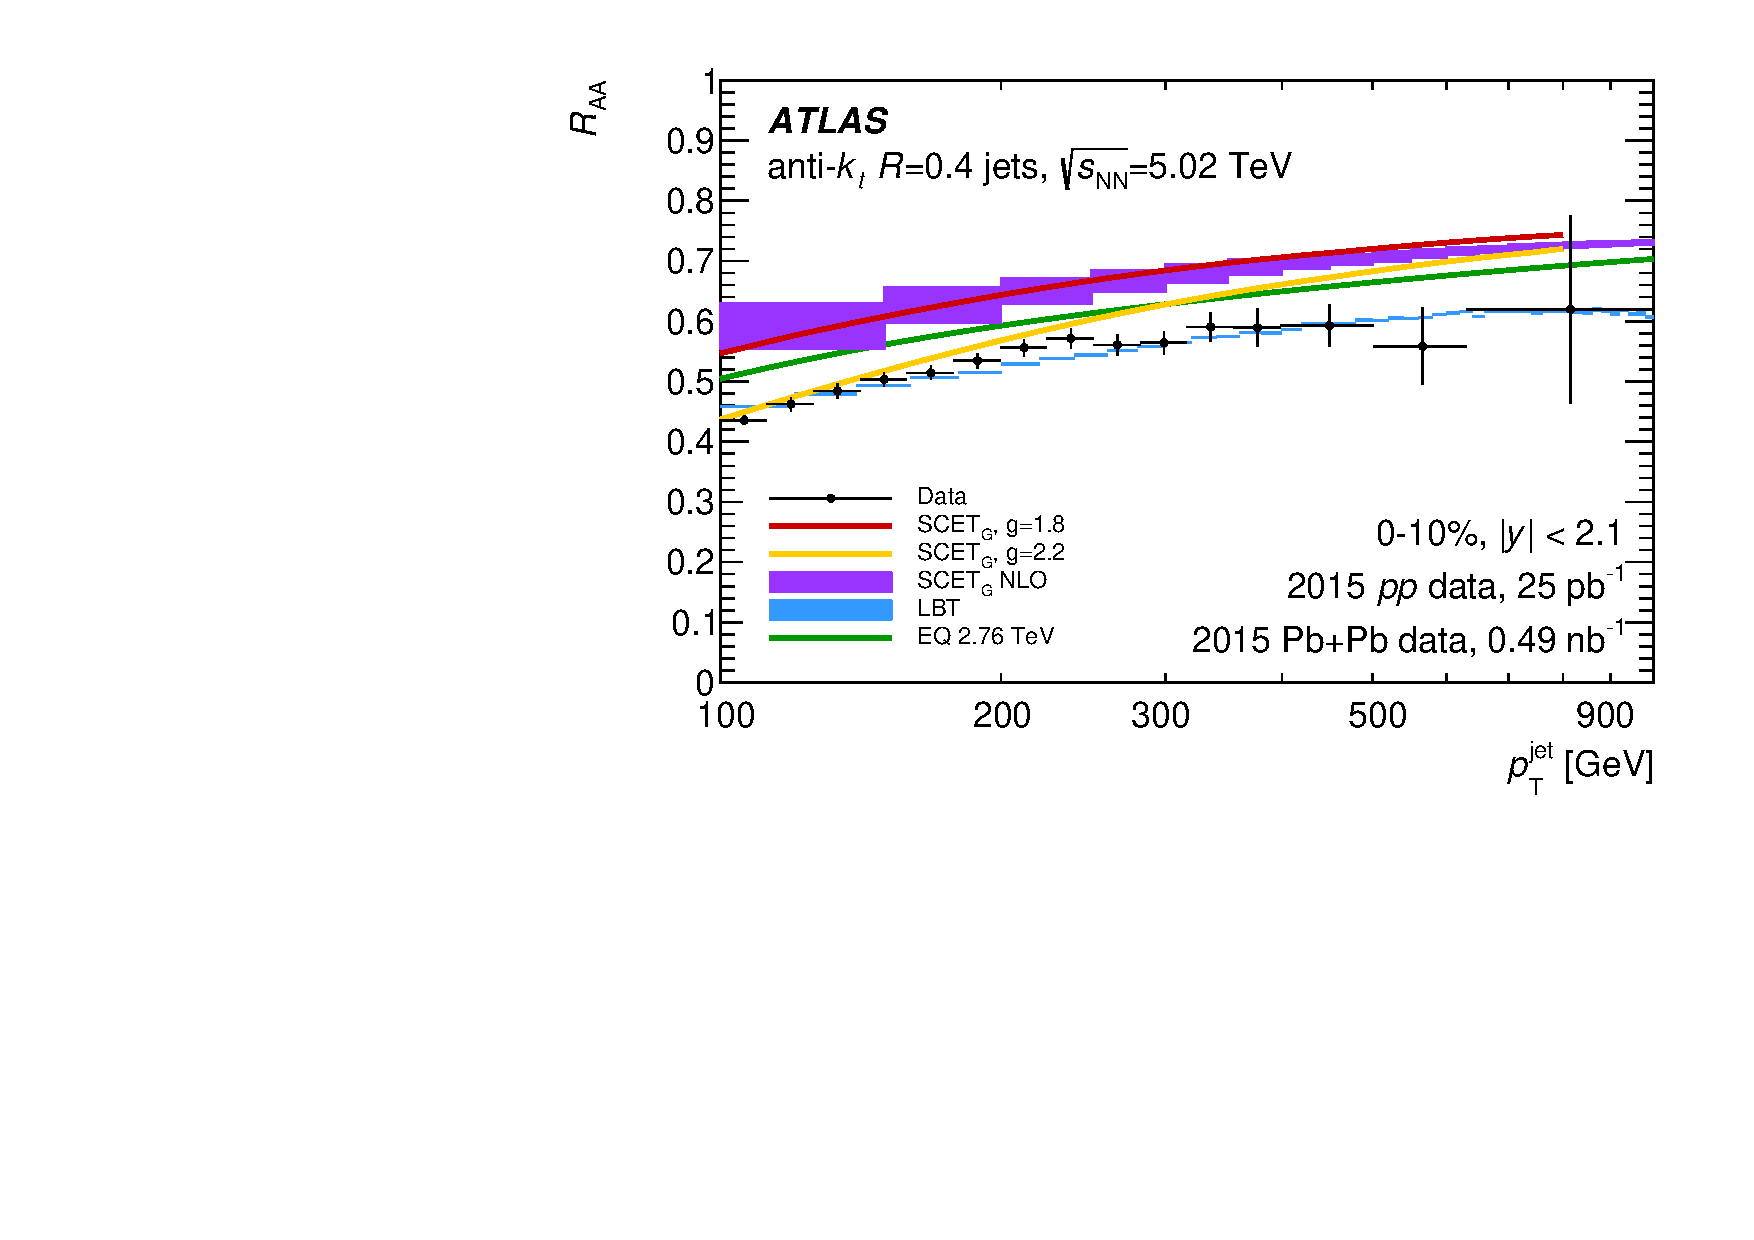
\includegraphics[width=0.65\textwidth]{fig/RAA_jet}\\
{\tiny  Figure is taken from {\color{teablue}
M.~Aaboud {\it et al.} [ATLAS Collaboration],
  %``Measurement of the nuclear modification factor for inclusive jets in Pb+Pb collisions at $\sqrt{s_\mathrm{NN}}=5.02$ TeV with the ATLAS detector,''
  Phys.\ Lett.\ B {\bf 790}, 108 (2019).
  }}
\end{center}
\vspace{4mm}
{\large It is broken:}
\vspace{2mm}
\begin{enumerate}
\item{small-$x$ evolution in QCD;}
\vspace{4mm}
\item{AdS/CFT.}
\end{enumerate}
\end{frame}
%
%%%%%%%%%%%%%%%%%%%%%%%%%%%%%%%%%%%%%%%%%%%%%%%%%%%%%%%%%%
%
\setcounter{page}{0}
\begin{frame}
\topskip0pt
\vspace*{\fill}
\begin{center}
{\Huge\bf\color{gray} Bulk in small systems}
\end{center}
\vspace*{\fill}
\end{frame}


%
%
%%%%%%%%%%%%%%%%%%%%%%%%%%%%%%%%%%%%%%%%%%%%%%%%%%%%%%%%%%
%
\begin{frame}{\bf\huge Hydro vs Non-hydro Modes}
\vspace{4mm}
\begin{itemize}
\item{\Large Two trivial statements:}\\
\vspace{4mm}
\begin{enumerate}
\item{\large QFTs contain hydrodynamics.}
\vspace{4mm}
\item{\color{darkred}\large QFTs go beyond hydrodynamics in different ways.}
\end{enumerate}
\vspace{4mm}
\item{\Large Examples:}
\end{itemize}
\begin{columns}
\begin{column}{0.45\textwidth}
\begin{center}
%\includegraphics[width=\textwidth]{omega_ADS}
\begin{overpic}[width=\textwidth]{fig/omega_ADS}
\put (30, -8){\color{teablue}cf. Saso's talk}
\end{overpic}
\end{center}
\end{column}
\begin{column}{0.45\textwidth}
%\setcounter{page}{2}
\begin{center}
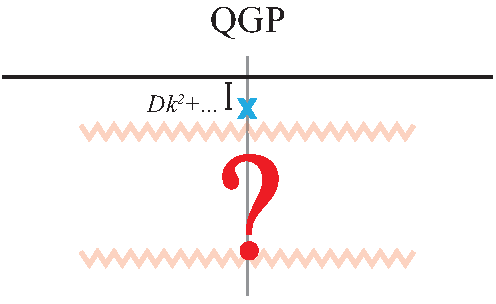
\includegraphics[width=\textwidth]{fig/omega_QCD}
\end{center}
\end{column}
\end{columns}
\vspace{4mm}
\begin{center}
the analytic structure of {\small $G_R^{\alpha\beta, \gamma\delta}(\omega, \vec{k}) = -i\int d^4 x e^{ik\cdot x}\theta(x^0)\langle[T^{\alpha\beta}(x),T^{\gamma\delta}(0)] \rangle$}
\end{center}
\end{frame}
%
%
%%%%%%%%%%%%%%%%%%%%%%%%%%%%%%%%%%%%%%%%%%%%%%%%%%%%%%%%%%
%
\begin{frame}{\bf\huge Strategy to Probe Inner Workings of QGP}
%\setcounter{page}{3}
\begin{center}
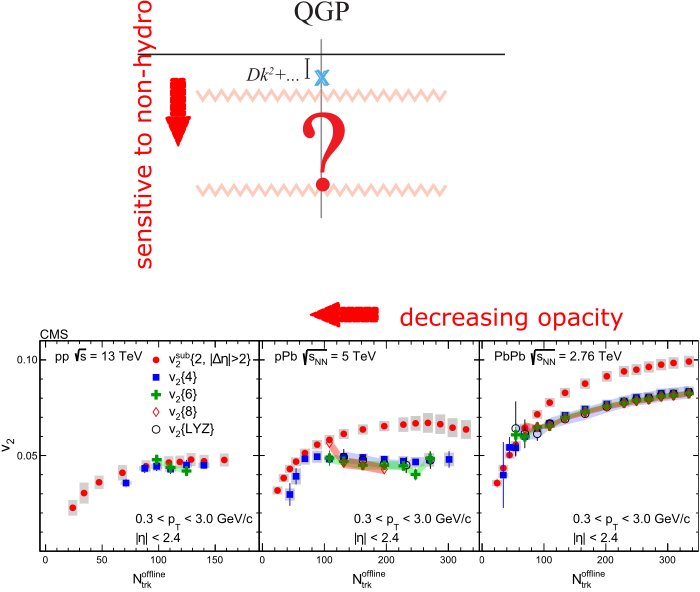
\includegraphics[width=0.7\textwidth]{fig/goal}
\vspace{2mm}\\
{\color{white}\bf\LARGE Decreasing $R\sim 1/k$ enhances non-hydro contributions.}
\end{center}
\end{frame}
%
%%%%%%%%%%%%%%%%%%%%%%%%%%%%%%%%%%%%%%%%%%%%%%%%%%%%%%%%%%
%
\begin{frame}{\bf\huge Strategy to Probe Inner Workings of QGP}
\begin{center}
\begin{overpic}[width=0.7\textwidth]{fig/goalo}
\put (25, 46){\color{black}\framebox[1.1\width]{$G_R(\tau, k)\sim {\color{hydroblue}c_{hyd} e^{-D k^2 \tau}} + {\color{red}\text{non-hydro terms}}$}}
\end{overpic}\vspace{2mm}\\
{\color{darkred}\bf\LARGE Decreasing $R\sim 1/k$ enhances non-hydro contributions.}
\end{center}
\end{frame}
%
%%%%%%%%%%%%%%%%%%%%%%%%%%%%%%%%%%%%%%%%%%%%%%%%%%%%%%%%%%
%
\begin{frame}
\setcounter{page}{0}
\topskip0pt
\vspace*{\fill}
\begin{center}
{\Huge\bf\color{gray} An Illustration Using A\\Conformal Kinetic Transport (CKT)}
\end{center}
\vspace*{\fill}
\end{frame}
%
%
%%%%%%%%%%%%%%%%%%%%%%%%%%%%%%%%%%%%%%%%%%%%%%%%%%%%%%%%%%
%
\begin{frame}{\bf\huge Hydro Is Hydro}
\setcounter{page}{5}
\vspace{4mm}
\begin{center}
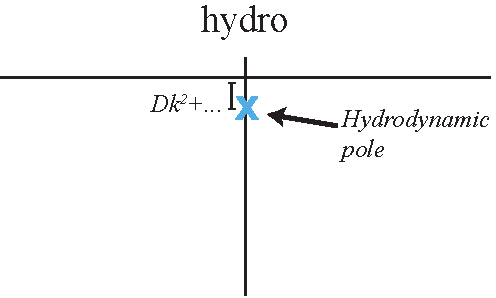
\includegraphics[width=0.6\textwidth]{fig/omega_hydro}
\end{center}
{\tiny  {\color{white} Romatschke,
  %``Retarded correlators in kinetic theory: branch cuts, poles and hydrodynamic onset transitions,''
  Eur.\ Phys.\ J.\ C {\bf 76}, no. 6, 352 (2016)
  %doi:10.1140/epjc/s10052-016-4169-7
  [arXiv:1512.02641];\\Kurkela and Wiedemann,
  %``Analytic structure of nonhydrodynamic modes in kinetic theory,''
  arXiv:1712.04376.
  }
  }\vspace{4mm}\\
%\phantom
{{\LARGE\bf\color{white}The Israel-Stewart (IS) hydro}}
\vspace{4mm}
\begin{center}
%\phantom
{\color{white}$D\Pi^{\mu\nu}+\frac{4}{3}\Pi^{\mu\nu}\nabla_\alpha u^\alpha = \frac{1}{\tau_\pi}\left(\Pi^{\mu\nu}+2 \eta\sigma^{\mu\nu}\right).$}
\end{center}
 \end{frame}
%
%
%%%%%%%%%%%%%%%%%%%%%%%%%%%%%%%%%%%%%%%%%%%%%%%%%%%%%%%%%%
%
\begin{frame}{\bf\huge IS Hydro Is Not Only Hydro}
\setcounter{page}{5}
\vspace{4mm}
\begin{center}
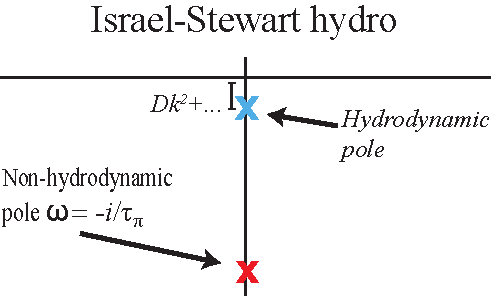
\includegraphics[width=0.6\textwidth]{fig/omega_IS}
\end{center}
{\tiny {\color{white} Romatschke,
  %``Retarded correlators in kinetic theory: branch cuts, poles and hydrodynamic onset transitions,''
  Eur.\ Phys.\ J.\ C {\bf 76}, no. 6, 352 (2016)
  %doi:10.1140/epjc/s10052-016-4169-7
  [arXiv:1512.02641];\\Kurkela and Wiedemann,
  %``Analytic structure of nonhydrodynamic modes in kinetic theory,''
  arXiv:1712.04376.
  }
  }\vspace{4mm}\\
%\phantom
{{\LARGE\bf\color{darkred} The Israel-Stewart (IS) hydro}}
%\setcounter{page}{5}
\vspace{4mm}
\begin{center}
%\phantom
{$D\Pi^{\mu\nu}+\frac{4}{3}\Pi^{\mu\nu}\nabla_\alpha u^\alpha = \frac{1}{\tau_\pi}\left(\Pi^{\mu\nu}+2 \eta\sigma^{\mu\nu}\right).$}
\end{center}
 \end{frame}
%
%
%%%%%%%%%%%%%%%%%%%%%%%%%%%%%%%%%%%%%%%%%%%%%%%%%%%%%%%%%%
%
\begin{frame}{\bf\huge Kinetic Transport in ITA Is Not Less Hydro}
%\setcounter{page}{6}
\vspace{2mm}
\begin{center}
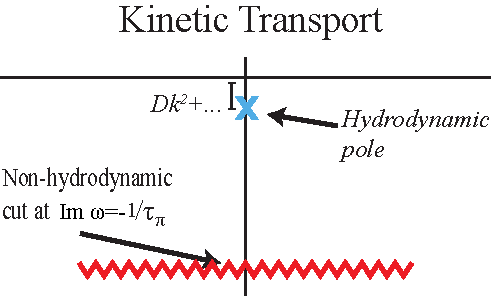
\includegraphics[width=0.6\textwidth]{fig/omega_RTA}
\end{center}
{\tiny  {\color{teablue} Romatschke,
  %``Retarded correlators in kinetic theory: branch cuts, poles and hydrodynamic onset transitions,''
  Eur.\ Phys.\ J.\ C {\bf 76}, no. 6, 352 (2016)
  %doi:10.1140/epjc/s10052-016-4169-7
  [arXiv:1512.02641]; Kurkela and Wiedemann,
  %``Analytic structure of nonhydrodynamic modes in kinetic theory,''
  arXiv:1712.04376.
  }
  }\vspace{4mm}\\
%\phantom
{{With the same transport coefficients and $\tau_\pi$ calculated in the CKT,}}
\vspace{4mm}
\begin{enumerate}
\item {The CKT and IS hydro have the same hydro pole.}
\vspace{4mm}
\item {\color{darkred}IS non-hydro pole is replaced by a branch cut in CKT.}
\end{enumerate}
%\vspace{4mm}
%\begin{center}
%\phantom
%{$ \partial_\tau f + \vec{v}_\perp \cdot \partial_{\vec{x}_\perp} f -\frac{p_z}{\tau}\partial_{p_z}f =-\frac{1}{\tau_{iso}}(-v_\mu u^{\mu})( f- f_{iso}).$}
%\end{center}
\end{frame}
%
%
%%%%%%%%%%%%%%%%%%%%%%%%%%%%%%%%%%%%%%%%%%%%%%%%%%%%%%%%%%
%
\begin{frame}{\bf\huge Features of the CKT}
%%\setcounter{page}{6}
\begin{center}
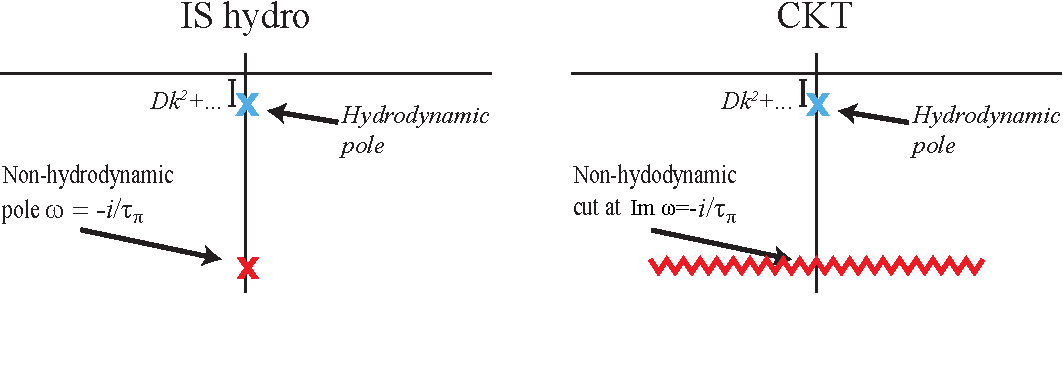
\includegraphics[width=0.8\textwidth]{fig/omega_ISCKT0}\end{center}
%\phantom
\begin{enumerate}
\item {Physics depends on only one dimensionless parameter:}\\
\begin{center}
{\color{darkred}
\framebox[1.1\width]{
Opacity: $\hat{\gamma} = \gamma R^{\frac{3}{4}} (\varepsilon_0 \tau_0)^{\frac{1}{4}}$
}
}
\end{center}
\item {CKT and IS hydro with (conformal EOS) have the same hydro pole.}
\item {The transport coefficients:}
$
\frac{\eta}{s} = \frac{1}{5}\frac{T}{\gamma \varepsilon^\frac{1}{4}}
$
\item {CFT interpolates free-streaming ($\hat{\gamma}\to 0$) and ideal hydro ($\hat{\gamma}\to\infty$)}
\item {\color{darkred}For $\tau_\pi = \frac{1}{\gamma \varepsilon^\frac{1}{4}}$, IS non-hydro pole degrades into a branch cut in CKT.}
\end{enumerate}
\end{frame}
%
%
%%%%%%%%%%%%%%%%%%%%%%%%%%%%%%%%%%%%%%%%%%%%%%%%%%%%%%%%%%
%
%\begin{frame}{\bf\huge Pin Down Sensitivity to Non-hydro Modes}
%\begin{center}
%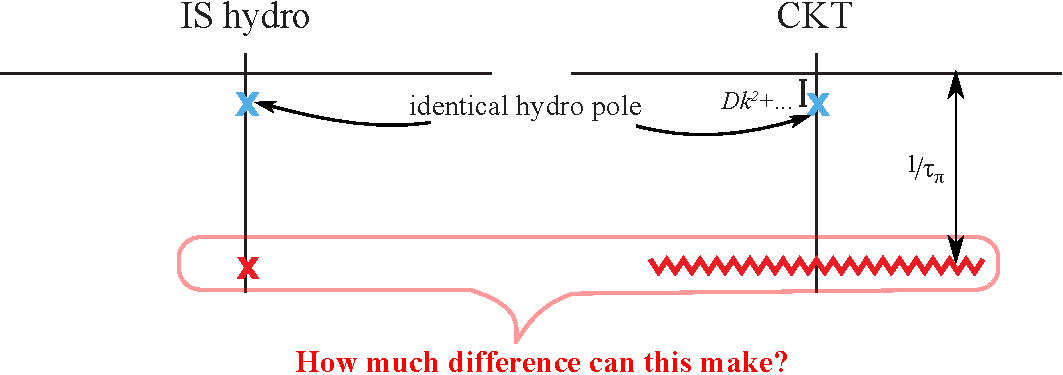
\includegraphics[width=0.8\textwidth]{fig/omega_ISCKT}\end{center}
%\vspace{4mm}
%The approach to answer this question:
%\vspace{4mm}
%\begin{center}
%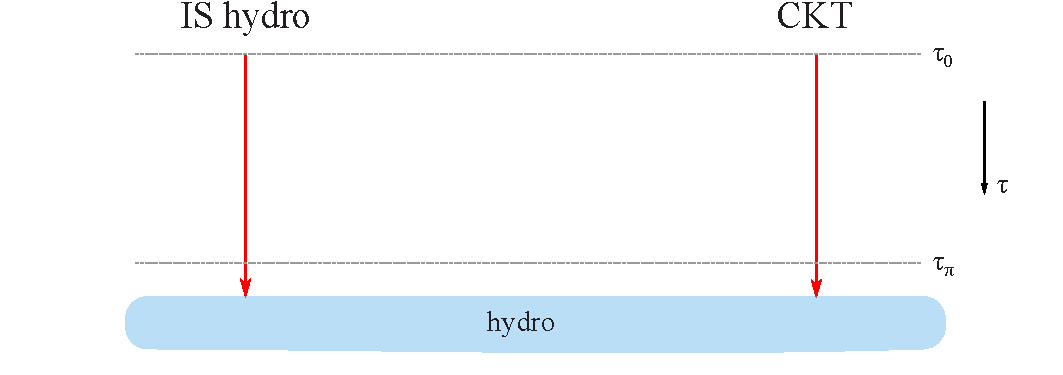
\includegraphics[width=0.8\textwidth]{fig/approachnonhydro}\end{center}
%%\phantom
%%\begin{enumerate}
%%\item {Physics depends on only one dimensionless parameter:}\\
%%\begin{center}
%%{\color{darkred}
%%\framebox[1.1\width]{
%%Opacity: $\hat{\gamma} = \gamma R^{\frac{3}{4}} (\varepsilon_0 \tau_0)^{\frac{1}{4}}$
%%}
%%}
%%\end{center}
%%\item {CKT and IS hydro with (conformal EOS) have the same hydro pole.}
%%\item {The transport coefficients:}
%%$
%%\frac{\eta}{s} = \frac{1}{5}\frac{T}{\gamma \varepsilon^\frac{1}{4}}
%%$
%%\item {CFT interpolates free-streaming ($\hat{\gamma}\to 0$) and ideal hydro ($\hat{\gamma}\to\infty$)}
%%\item {\color{darkred}For $\tau_\pi = \frac{1}{\gamma \varepsilon^\frac{1}{4}}$, IS non-hydro pole degrades into a branch cut in CKT.}
%%\end{enumerate}
%\end{frame}
%
%%%%%%%%%%%%%%%%%%%%%%%%%%%%%%%%%%%%%%%%%%%%%%%%%%%%%%%%%%
%
\begin{frame}{\bf\huge Pin Down Sensitivity to Non-hydro Modes}
%\setcounter{page}{7}
\begin{center}
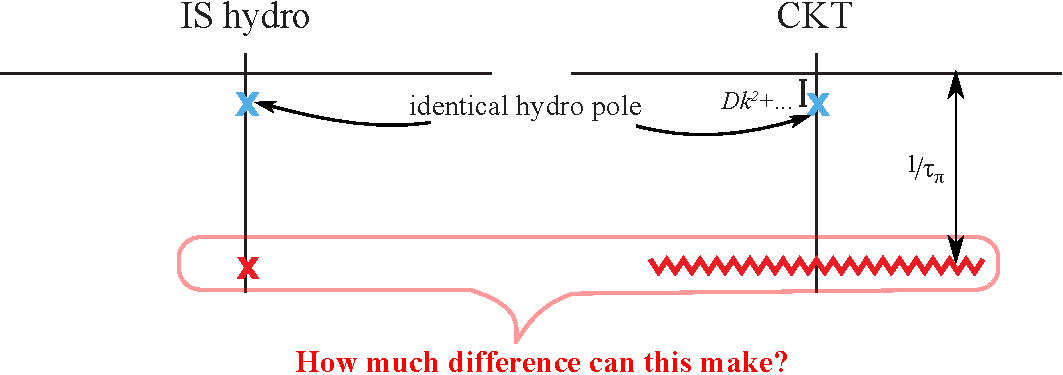
\includegraphics[width=0.8\textwidth]{fig/omega_ISCKT}\end{center}
\vspace{4mm}
The approach to answer this question:
\vspace{4mm}
\begin{center}
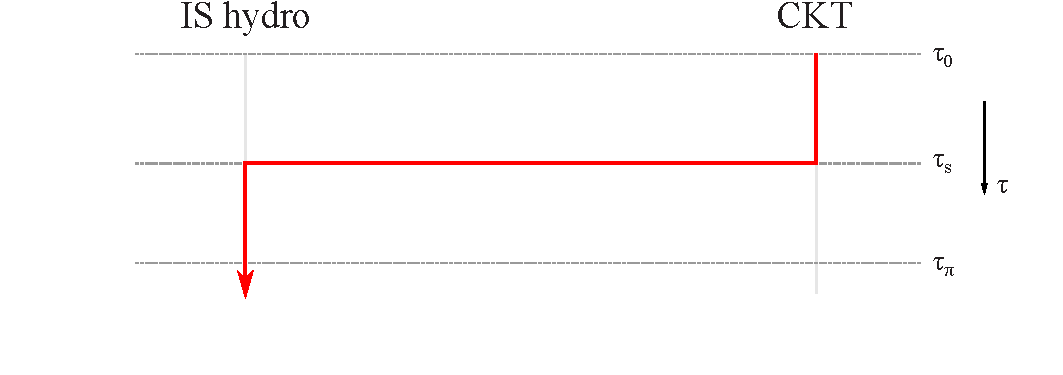
\includegraphics[width=0.8\textwidth]{fig/approachnonhydros}\end{center}
%\phantom
%\begin{enumerate}
%\item {Physics depends on only one dimensionless parameter:}\\
%\begin{center}
%{\color{darkred}
%\framebox[1.1\width]{
%Opacity: $\hat{\gamma} = \gamma R^{\frac{3}{4}} (\varepsilon_0 \tau_0)^{\frac{1}{4}}$
%}
%}
%\end{center}
%\item {CKT and IS hydro with (conformal EOS) have the same hydro pole.}
%\item {The transport coefficients:}
%$
%\frac{\eta}{s} = \frac{1}{5}\frac{T}{\gamma \varepsilon^\frac{1}{4}}
%$
%\item {CFT interpolates free-streaming ($\hat{\gamma}\to 0$) and ideal hydro ($\hat{\gamma}\to\infty$)}
%\item {\color{darkred}For $\tau_\pi = \frac{1}{\gamma \varepsilon^\frac{1}{4}}$, IS non-hydro pole degrades into a branch cut in CKT.}
%\end{enumerate}
\end{frame}
%
%%%%%%%%%%%%%%%%%%%%%%%%%%%%%%%%%%%%%%%%%%%%%%%%%%%%%%%%%%
%
\begin{frame}{\bf\huge Proof of Sensitivity to Non-hydro Modes}
\begin{center}
\begin{overpic}[width=0.7\textwidth]{fig/ckthydro}
%\put (25, 46){\color{darkred}$G_R(t, k)\sim c_{hyd} e^{-D k^2 t} + \text{non-hydro terms}$}
\end{overpic}\vspace{4mm}\\
{\color{darkred}\bf\LARGE Sensitivity to non-hydro modes is more pronounced in small systems.}
\vspace{4mm}\\
{\tiny  {\color{teablue} Kurkela, Wiedemann and BW,
  %``Kinetic transport is needed to reliably extract shear viscosity from pA and AA data,''
  arXiv:1805.04081.
  }
  }
\end{center}
\end{frame}
%
%%%%%%%%%%%%%%%%%%%%%%%%%%%%%%%%%%%%%%%%%%%%%%%%%%%%%%%%%%
%
\begin{frame}{\bf\huge Interpretation of Sensitivity to Non-hydro Modes}
\begin{center}
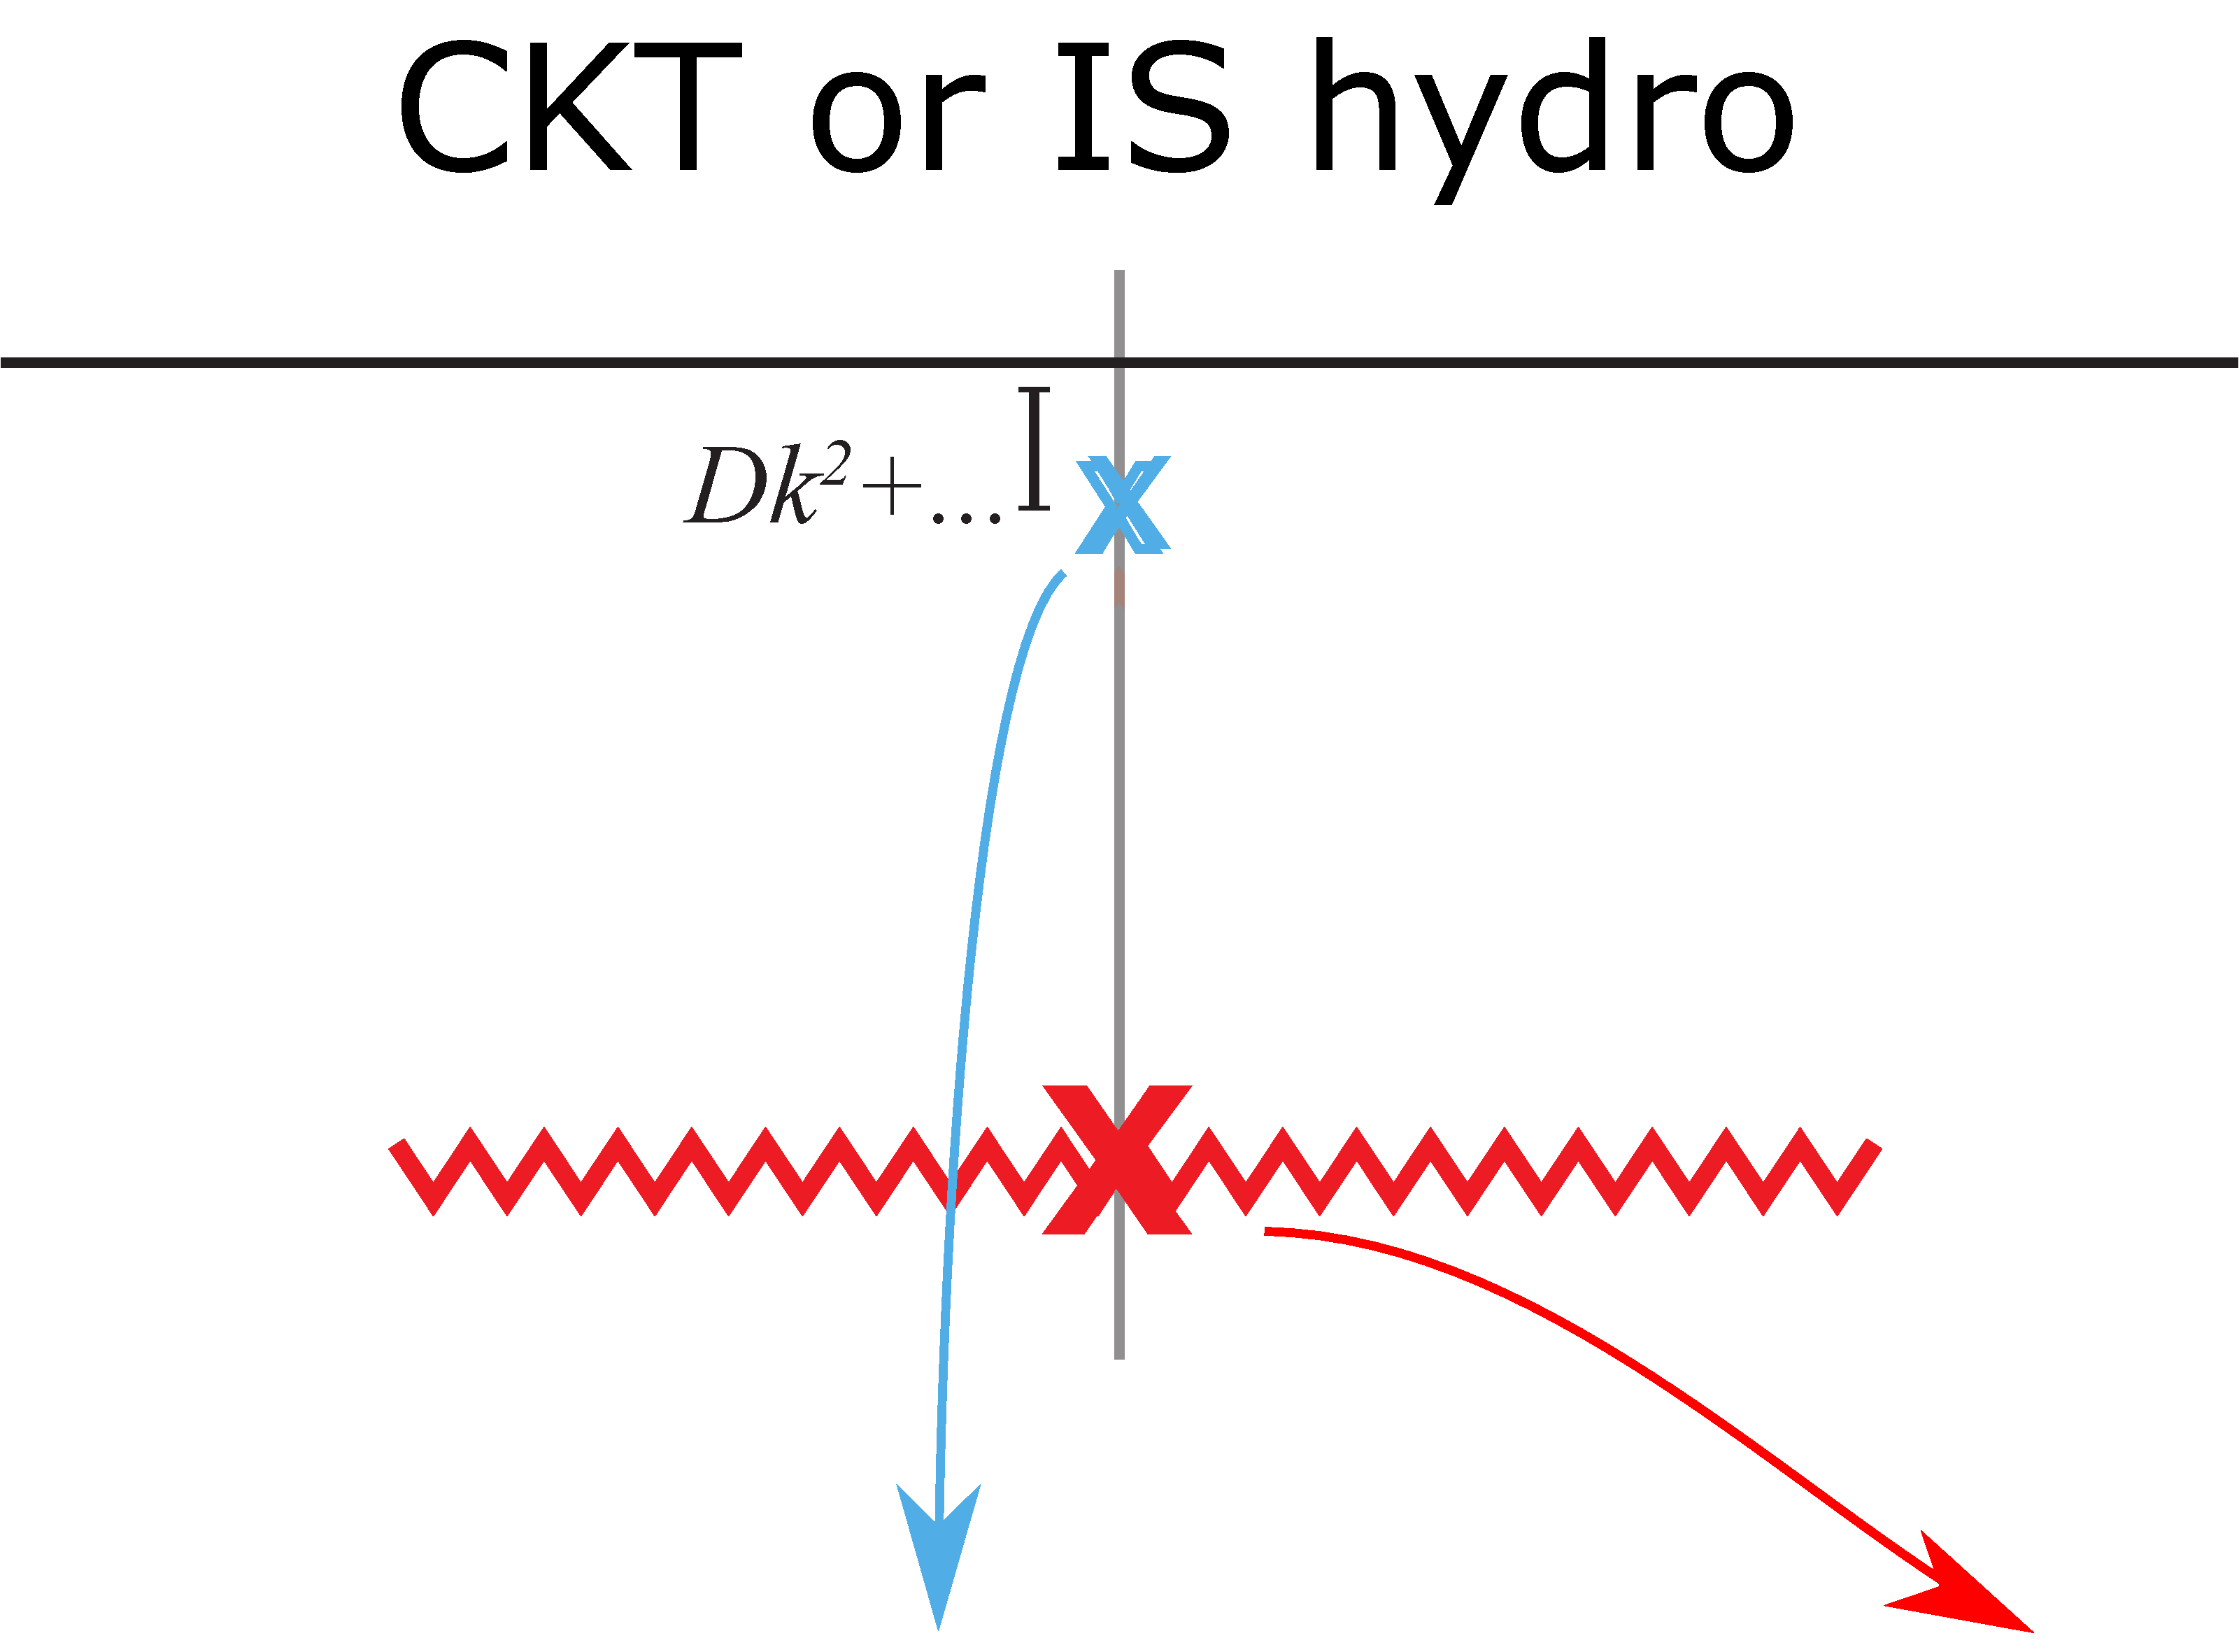
\includegraphics[width=0.5\textwidth]{fig/CKTIS}
\vspace{2mm}
\\
{\color{black}\framebox[1.1\width]{\bm $G_R(\tau, k)\sim {\color{hydroblue}c_{hyd} \underbrace{e^{-D k^2 \tau}}_{\text{reduced for small $R$}}} + {\color{red}c_{non-hyd} \underbrace{e^{-\frac{\tau}{\tau_\pi}}}_{\text{enhanced for small $\varepsilon$}}}$}}
\\\vspace{10mm}
{\color{darkred}\LARGE Non-hydro modes are enhanced in small or dilute systems $\Leftrightarrow$ small $\hat\gamma= R/l_{mfp}$ with $l_{mfp}$ mean free path.}
\end{center}
\end{frame}
%
%%%%%%%%%%%%%%%%%%%%%%%%%%%%%%%%%%%%%%%%%%%%%%%%%%%%%%%%%%
%
\begin{frame}{\bf\huge Flow PURELY from Non-hydro modes at $\hat{\gamma}\to0$}
\vspace{4mm}
{{\LARGE From mode-mode coupling due to \color{darkred}  one final-state scattering}}
\vspace{2mm}
{
\begin{eqnarray}
 \frac{d E_\perp}{d \eta d \phi}
= \frac{1}{2\pi}\frac{d E_\perp}{d \eta}\Big\vert_{\hat\gamma=0,\epsilon_n =0} 
&&  \left\{
1 -0.210 \,\hat\gamma -{\color{darkred} \underbrace{0.212 \, \hat\gamma \epsilon_2}_{v_2}} \, 2 \cos(2 \phi - 2 \psi_2) \right.\nonumber \\
&& -{\color{darkred} \underbrace{ 0.140 \,\hat\gamma \epsilon_3}_{v_3}} \, 2 \cos(3\phi- 3\psi_3)\nonumber \\
&&+ {\color{darkred} \underbrace{0.063 \,\hat\gamma \epsilon_2^2}_{v_4}} 2 \cos(4 \phi - 4 \psi_2) +0.015\, \hat\gamma \epsilon_2^2\nonumber \\
&& +{\color{darkred} \underbrace{0.112\, \hat\gamma \epsilon_3^2}_{v_6}} 2 \cos(6 \phi - 6 \psi_3) + 0.043 \,\hat\gamma \epsilon_3^2 \nonumber \\
&&\left.+ {\color{darkred} \underbrace{0.088 \,\hat\gamma \epsilon_2 \epsilon_3}_{v_5}} 2 \cos(5\phi - 3\psi_3- 2\psi_2)
 \right\}\,\nonumber.
\end{eqnarray}
}
\vspace{1mm}
\begin{center}
{\tiny  {\color{teablue} Kurkela, Wiedemann and BW,
  %``Kinetic transport is needed to reliably extract shear viscosity from pA and AA data,''
  Phys.\ Lett.\ B {\bf 783}, 274 (2018), [arXiv:1803.02072].
  }
  }
\end{center}
\end{frame}
%
%%%%%%%%%%%%%%%%%%%%%%%%%%%%%%%%%%%%%%%%%%%%%%%%%%%%%%%%%%
%
\setcounter{page}{8}
\begin{frame}{\bf\huge Physical picture for flow in small systems}
\vspace{4mm}
\begin{center}
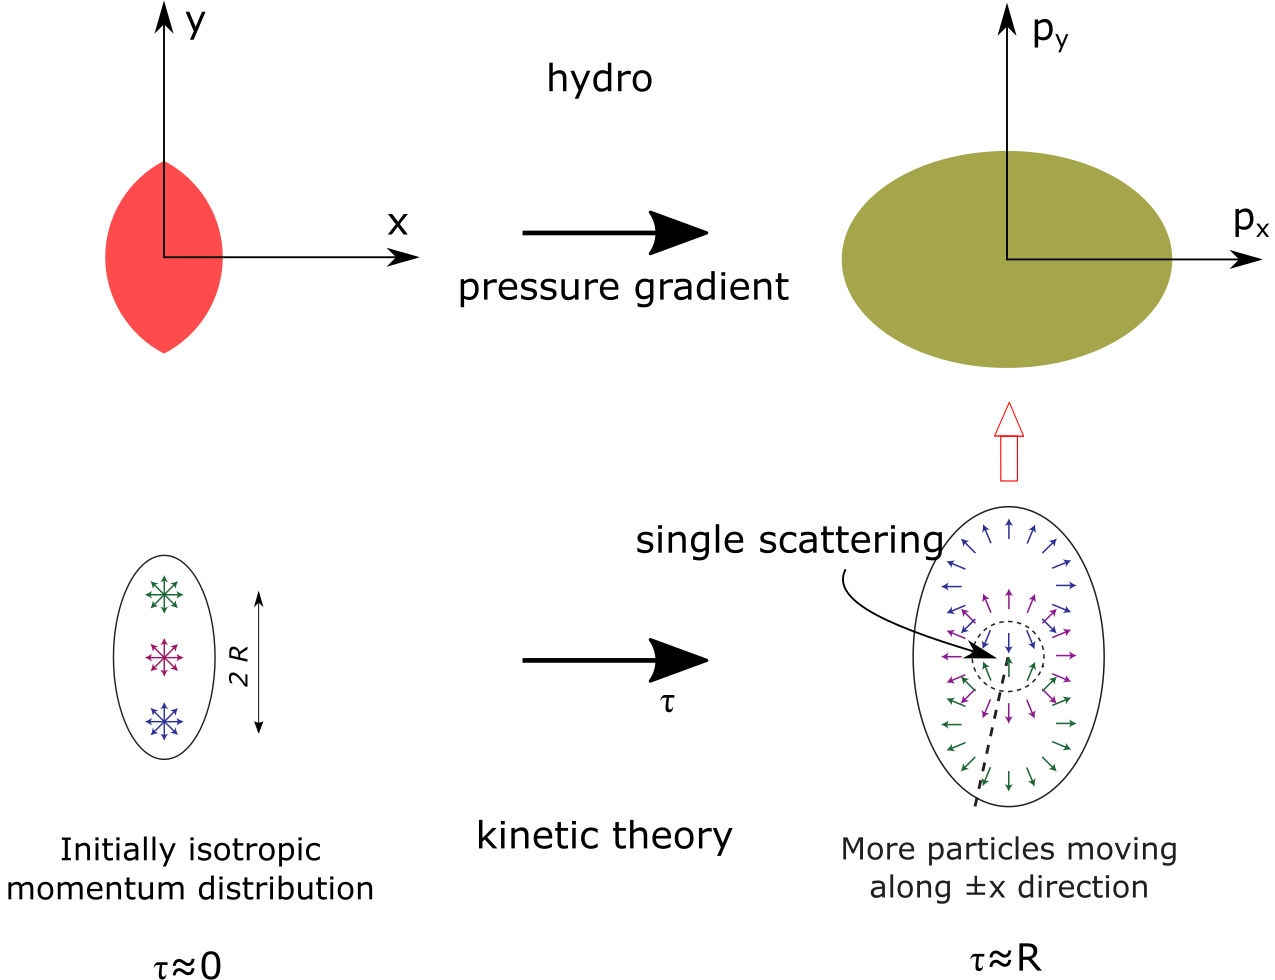
\includegraphics[width=0.65\textwidth]{fig/onehit}\\
{\tiny  {\color{teablue} Kurkela, Wiedemann and BW,
  %``Kinetic transport is needed to reliably extract shear viscosity from pA and AA data,''
  Phys.\ Lett.\ B {\bf 783}, 274 (2018), [arXiv:1803.02072].
  }
  }
\end{center}
\vspace{4mm}
{{\LARGE\color{darkred} Flow is a signature for final-state interactions, not for hydro!}}
\vspace{2mm}\\
{\tiny  See also: {\color{teablue}   Borghini \& Gombeaud,
  %``Anisotropic flow far from equilibrium,''
  Eur.\ Phys.\ J.\ C {\bf 71} (2011) 1612; He, Edmonds, Lin, Liu, Molnar \& Wang,
  %``Anisotropic parton escape is the dominant source of azimuthal anisotropy in transport models,''
  Phys.\ Lett.\ B {\bf 753} (2016) 506.
  }
}
\end{frame}
%
%%%%%%%%%%%%%%%%%%%%%%%%%%%%%%%%%%%%%%%%%%%%%%%%%%%%%%%%%%
%
\begin{frame}{\bf\huge From Free-streaming to Ideal Hydro}
\begin{center}
\begin{overpic}[width=0.7\textwidth]{fig/ckthydrofull}
%\put (25, 46){\color{darkred}$G_R(t, k)\sim c_{hyd} e^{-D k^2 t} + \text{non-hydro terms}$}
\end{overpic}\vspace{4mm}\\
{\color{darkred}\bf\LARGE Non-hydro modes are more efficient to build up $v_2$ in small systems!}
\vspace{4mm}\\
{\tiny  {\color{teablue} Kurkela, Wiedemann and BW,
  %``Kinetic transport is needed to reliably extract shear viscosity from pA and AA data,''
  arXiv:1805.04081.
  }
  }
\end{center}
\end{frame}
%
%%%%%%%%%%%%%%%%%%%%%%%%%%%%%%%%%%%%%%%%%%%%%%%%%%%%%%%%%%
%
\begin{frame}
\setcounter{page}{0}
\topskip0pt
\vspace*{\fill}
\begin{center}
{\Huge\bf\color{gray} Hydro vs Non-hydro}
\end{center}
\vspace*{\fill}
\end{frame}
\setcounter{page}{13}
%
%
%%%%%%%%%%%%%%%%%%%%%%%%%%%%%%%%%%%%%%%%%%%%%%%%%%%%%%%%%%
%

\begin{frame}{\bf\huge Qualification of Being a Fluid}
%\setcounter{page}{6}
\vspace{4mm}
{\color{darkred}\bf\LARGE Criteria:}
\vspace{4mm}
\begin{center}
{\huge\color{darkred}
\framebox[0.5\textwidth]{hydro-like $\Leftrightarrow Q<0.1$}
}
\end{center}
\vspace{4mm}
{\Large \color{black} in terms of  ''fluid quality''}
\begin{center}
{\Large\color{black}
%\framebox[1.1\width]
{
$Q(t,r) =  \sqrt{  \frac{ \left( T_{\rm kin}- T_{\rm hyd} \right)^{\mu\nu}   \left( T_{\rm kin} - T_{\rm hyd} \right)_{\mu\nu} }{ \left(T_{\rm id} \right)^{\mu\nu}    \left(T_{\rm id} \right)_{\mu\nu}    }  }.$
}
}
\vspace{2mm}\\
{\tiny  {\color{teablue} Kurkela, Wiedemann and BW, arXiv:1905.05139.
%doi:10.1088/1126-6708/2008/04/100
%[arXiv:0712.2451].
  }
  }
\end{center}
\vspace{2mm}
{\color{black}\Large Up to 2nd order in gradient expansion, }
\begin{align}
&T_{\rm hyd}^{\mu\nu} = \left( \varepsilon + p\right) u^\mu\, u^\nu + p\, g^{\mu\nu} + \Pi^{\mu\nu}_{\rm hyd}\nonumber\\
&\Pi^{\mu\nu}_{\rm hyd} = - 2 \eta \sigma^{\mu\nu}+ 2 \tau_{\Pi}\, \eta \left[ ^<D\sigma^{\mu\nu>} 
	+ \frac{1}{3} \sigma^{\mu\nu} \nabla_\alpha u^\alpha \right] +	\lambda_1 \sigma^{<\mu}_\alpha\, \sigma^{\nu> \lambda} \nonumber\\
&\sigma^{\mu\nu} =  \left\{\frac{1}{2}\left[ \Delta^{\mu\alpha} \nabla_\alpha u^\nu {+} \Delta^{\nu\alpha} \nabla_\alpha u^\mu \right] 
				{-} \frac{1}{3}\Delta^{\mu\nu} \nabla_\alpha u^\alpha \right\}\nonumber
\end{align}
\begin{center}
\vspace{2mm}
{\tiny  {\color{teablue}   Baier, Romatschke, Son, Starinets and Stephanov,
  %``Relativistic viscous hydrodynamics, conformal invariance, and holography,''
  JHEP {\bf 0804}, 100 (2008).
%doi:10.1088/1126-6708/2008/04/100
%[arXiv:0712.2451].
  }
  }
  \end{center}
\end{frame}
%
%%%%%%%%%%%%%%%%%%%%%%%%%%%%%%%%%%%%%%%%%%%%%%%%%%%%%%%%%%
%
\begin{frame}{\bf\huge How Much "Fluid" is CKT?}
\vspace{4mm}
\begin{center}
\begin{overpic}[width=1\textwidth]{fig/Q1}
%\put (25, 46){\color{darkred}$G_R(t, k)\sim c_{hyd} e^{-D k^2 t} + \text{non-hydro terms}$}
\end{overpic}
%\vspace{4mm}\\
%{\Large {\color{nonhydroregion}\framebox[0.3\textwidth]{particle-like: $\hat{\gamma}\lesssim 2$}} {\color{transregion}\framebox[0.33\textwidth]{transition: $4\lesssim\hat{\gamma}\lesssim 2$}} {\color{hydroregion}\framebox[0.3\textwidth]{hydro-like: $\hat{\gamma}\gtrsim 4$}}}
\vspace{1mm}\\
{\tiny  {\color{teablue} Kurkela, Wiedemann and BW, arXiv:1905.05139.
%doi:10.1088/1126-6708/2008/04/100
%[arXiv:0712.2451].
  }
  }
\end{center}
\end{frame}
%
%%%%%%%%%%%%%%%%%%%%%%%%%%%%%%%%%%%%%%%%%%%%%%%%%%%%%%%%%%
%
\begin{frame}{\bf\huge How Much "Fluid" is CKT?}
\setcounter{page}{14}
\vspace{4mm}
\begin{center}
\begin{overpic}[width=1\textwidth]{fig/Q1Q}
%\put (25, 46){\color{darkred}$G_R(t, k)\sim c_{hyd} e^{-D k^2 t} + \text{non-hydro terms}$}
\end{overpic}
%\vspace{4mm}\\
%{\Large {\color{nonhydroregion}\framebox[0.3\textwidth]{particle-like: $\hat{\gamma}\lesssim 2$}} {\color{transregion}\framebox[0.33\textwidth]{transition: $4\lesssim\hat{\gamma}\lesssim 2$}} {\color{hydroregion}\framebox[0.3\textwidth]{hydro-like: $\hat{\gamma}\gtrsim 4$}}}
\vspace{1mm}\\
{\tiny  {\color{teablue} Kurkela, Wiedemann and BW, arXiv:1905.05139.
%doi:10.1088/1126-6708/2008/04/100
%[arXiv:0712.2451].
  }
  }
\end{center}
\end{frame}
%
%%%%%%%%%%%%%%%%%%%%%%%%%%%%%%%%%%%%%%%%%%%%%%%%%%%%%%%%%%
%
\begin{frame}{\bf\huge How Much "Fluid" is CKT?}
\setcounter{page}{14}
\vspace{4mm}
\begin{center}
\begin{overpic}[width=1\textwidth]{fig/Q12}
%\put (25, 46){\color{darkred}$G_R(t, k)\sim c_{hyd} e^{-D k^2 t} + \text{non-hydro terms}$}
\end{overpic}
%\vspace{4mm}\\
%{\Large {\color{nonhydroregion}\framebox[0.3\textwidth]{particle-like: $\hat{\gamma}\lesssim 2$}} {\color{transregion}\framebox[0.33\textwidth]{transition: $4\lesssim\hat{\gamma}\lesssim 2$}} {\color{hydroregion}\framebox[0.3\textwidth]{hydro-like: $\hat{\gamma}\gtrsim 4$}}}
\vspace{1mm}\\
{\tiny  {\color{teablue} Kurkela, Wiedemann and BW, arXiv:1905.05139.
%doi:10.1088/1126-6708/2008/04/100
%[arXiv:0712.2451].
  }
  }
\end{center}
\end{frame}
%
%%%%%%%%%%%%%%%%%%%%%%%%%%%%%%%%%%%%%%%%%%%%%%%%%%%%%%%%%%
%
\begin{frame}{\bf\huge How Much "Fluid" is CKT?}
\setcounter{page}{14}
\vspace{4mm}
\begin{center}
\begin{overpic}[width=1\textwidth]{fig/Q12Q}
%\put (25, 46){\color{darkred}$G_R(t, k)\sim c_{hyd} e^{-D k^2 t} + \text{non-hydro terms}$}
\end{overpic}
%\vspace{4mm}\\
%{\Large {\color{nonhydroregion}\framebox[0.3\textwidth]{particle-like: $\hat{\gamma}\lesssim 2$}} {\color{transregion}\framebox[0.33\textwidth]{transition: $4\lesssim\hat{\gamma}\lesssim 2$}} {\color{hydroregion}\framebox[0.3\textwidth]{hydro-like: $\hat{\gamma}\gtrsim 4$}}}
\vspace{1mm}\\
{\tiny  {\color{teablue} Kurkela, Wiedemann and BW, arXiv:1905.05139.
%doi:10.1088/1126-6708/2008/04/100
%[arXiv:0712.2451].
  }
  }
\end{center}
\end{frame}
%
%%%%%%%%%%%%%%%%%%%%%%%%%%%%%%%%%%%%%%%%%%%%%%%%%%%%%%%%%%
%
\begin{frame}{\bf\huge Fluid vs Non-fluid in Our Numerical Results}
\vspace{4mm}
\begin{center}
\begin{overpic}[width=0.9\textwidth]{fig/hydroness}
%\put (25, 46){\color{darkred}$G_R(t, k)\sim c_{hyd} e^{-D k^2 t} + \text{non-hydro terms}$}
\end{overpic}
%\vspace{4mm}\\
%{\color{darkred}\bf\LARGE How to qualify how much ''fluid'' bulk matter is?}
%\vspace{4mm}\\
%{\small  {\color{teablue} Kurkela, Wiedemann and BW,
%   arXiv:1905.05139.
%  }
%  }
\end{center}
\end{frame}

%
%%%%%%%%%%%%%%%%%%%%%%%%%%%%%%%%%%%%%%%%%%%%%%%%%%%%%%%%%%
%
\begin{frame}
\setcounter{page}{0}
\topskip0pt
\vspace*{\fill}
\begin{center}
{\Huge\bf\color{gray} Confronting Data}
\end{center}
\vspace*{\fill}
\end{frame}
%
%%%%%%%%%%%%%%%%%%%%%%%%%%%%%%%%%%%%%%%%%%%%%%%%%%%%%%%%%%
%
\begin{frame}{\bf\huge Measurement of Opacity}
\setcounter{page}{16}
\vspace{4mm}
\begin{center}
\begin{overpic}[width=0.6\textwidth]{fig/v2ALICEvsKinThTeV5gamma}
%\put (10, 60){\color{darkred}a loose constraint: $\frac{\eta}{s}\in (2-4)/(4\pi)$}
\end{overpic}\\
{\tiny  GGMLO: {\color{teablue} Giacalone, Guerrero-Rodríguez, Luzum, Marquet \& Ollitrault,
  %``New paradigm for fluctuations in heavy-ion collisions,''
  arXiv:1902.07168.
  }
  }
\end{center}
\begin{enumerate}
\item {Definition: \color{teablue}\framebox[0.5\textwidth]{$\hat{\gamma}\equiv \gamma R (\varepsilon_0\tau_0/R)^\frac{1}{4}=\frac{0.11}{\eta/s} \left(\frac{R {\color{darkred} \frac{dE_\perp}{d\eta_s}}}{\pi f_{work}(\hat{\gamma})}\right)^\frac{1}{4}$}}\\
\vspace{2mm}
\item {Conformal scaling property:}
{\color{teablue}\framebox[0.35\textwidth]{$\left.\frac{v_2}{\epsilon_2}\right|_{\hat{\gamma}<1}\propto\left( R {\color{darkred}\langle p_\perp\rangle \frac{dN}{d\eta_s}}\right)^\frac{1}{4}$}
}
\end{enumerate}
\end{frame}
%
%%%%%%%%%%%%%%%%%%%%%%%%%%%%%%%%%%%%%%%%%%%%%%%%%%%%%%%%%%
%
\begin{frame}{\bf\huge Confronting AA Data}
\vspace{4mm}
\begin{center}
\begin{overpic}[width=\textwidth]{fig/GhatVScentPbPb502TeV}
%\put (20, 46){\color{darkred}$\Leftrightarrow$  evaluate $\hat{\gamma}$ from measurements!}
\end{overpic}
\end{center}
\vspace{2mm}
\begin{center}
{\color{black}($v_2$ gives a loose constraint on $4 \pi \frac{\eta}{s}\in (2, 4)$}.)
\end{center}
\vspace{6mm}
{{\LARGE\bf\color{darkred} Flow in (central) AA collisions is of hydro origin.}}
\vspace{6mm}
\begin{center}
{{\color{teablue}For details, cf. Urs' Talk}
}
\end{center}
\end{frame}
%
%%%%%%%%%%%%%%%%%%%%%%%%%%%%%%%%%%%%%%%%%%%%%%%%%%%%%%%%%%
%
\begin{frame}{\bf\huge Confronting pA Data}
\vspace{4mm}
\begin{center}
\begin{overpic}[width=\textwidth]{fig/GhatVScent502TeVpPb}
%\put (20, 46){\color{darkred}$\Leftrightarrow$  evaluate $\hat{\gamma}$ from measurements!}
\end{overpic}
\end{center}
\vspace{6mm}
{{\LARGE\bf\color{darkred} 
Flow in pA collisions mostly has a non-hydro origin because bulk matter is mostly not hydro-like.
%Flow measurements in pp, pA and AA collisions can be used to reveal inner workings of QGP beyond hydro.
}}
\vspace{6mm}
\begin{center}
{{\color{teablue}For details, cf. Urs' Talk}
}
\end{center}
\end{frame}
%
%%%%%%%%%%%%%%%%%%%%%%%%%%%%%%%%%%%%%%%%%%%%%%%%%%%%%%%%%%
%
\begin{frame}{\bf\huge Conclusions}
\setcounter{page}{0}
\vspace{4mm}
%\begin{enumerate}
{\color{teablue}1.} {\color{darkred}Probing inner workings of QGP $\Leftrightarrow$ going beyond hydrodynamics.}\\
\vspace{4mm}
{\color{teablue}2.} {\color{darkred} The strategy to do so is as follows:}\\
\vspace{2mm}
%\end{enumerate}
\begin{center}
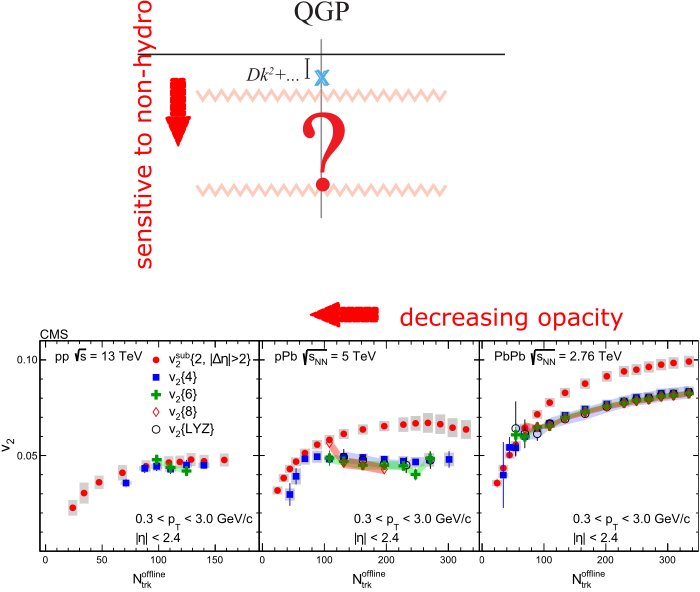
\includegraphics[width=0.6\textwidth]{fig/goal}
\end{center}
\end{frame}
%
%%%%%%%%%%%%%%%%%%%%%%%%%%%%%%%%%%%%%%%%%%%%%%%%%%%%%%%%%%
%
\begin{frame}{\bf\huge Conclusions}
\setcounter{page}{0}
\vspace{2mm}
{\color{teablue}3.} {\color{darkred}The CKT implements the same hydro as IS hydro with a physically motivated non-hydro sector. And we find}\\
\vspace{2mm}
\begin{center}
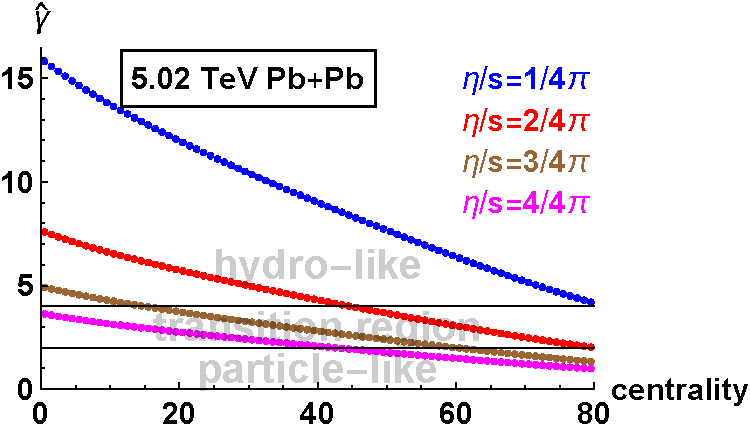
\includegraphics[width=0.4\textwidth]{fig/PbPb}\hspace{0.1\textwidth}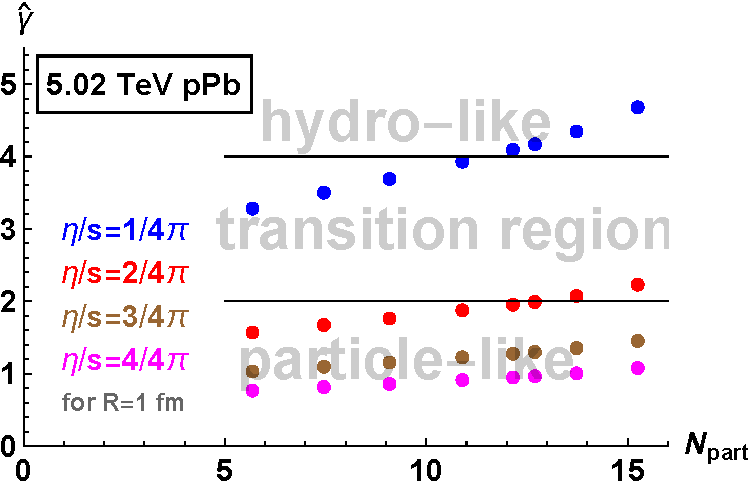
\includegraphics[width=0.4\textwidth]{fig/pPb}
\end{center}
\vspace{2mm}
And for small systems: {\color{darkred}\framebox[0.4\textwidth]{$\left.\frac{v_2}{\epsilon_2}\right|_{\hat{\gamma}<1}\propto\hat{\gamma}\propto\left( R \langle p_\perp\rangle \frac{dN}{d\eta_s}\right)^\frac{1}{4}$}
}\\
\vspace{4mm}
{\color{teablue}4.} {\color{darkred} The strategy provides a general approach \& implementation in all theories beyond hydro is most welcome.}
\end{frame}
%
%%%%%%%%%%%%%%%%%%%%%%%%%%%%%%%%%%%%%%%%%%%%%%%%%%%%%%%%%%
%
\begin{frame}
\setcounter{page}{0}
\topskip0pt
\vspace*{\fill}
\begin{center}
{\Huge\bf\color{gray}Backup Slides}
\end{center}
\vspace*{\fill}
\end{frame}
%
%
%%%%%%%%%%%%%%%%%%%%%%%%%%%%%%%%%%%%%%%%%%%%%%%%%%%%%%%%%%
%
\begin{frame}{\bf\huge Implementation in QFT}
\setcounter{page}{0}
{\color{darkred}QFT has richer structures than kinetic theory. In two-point function, one has}
\begin{center}
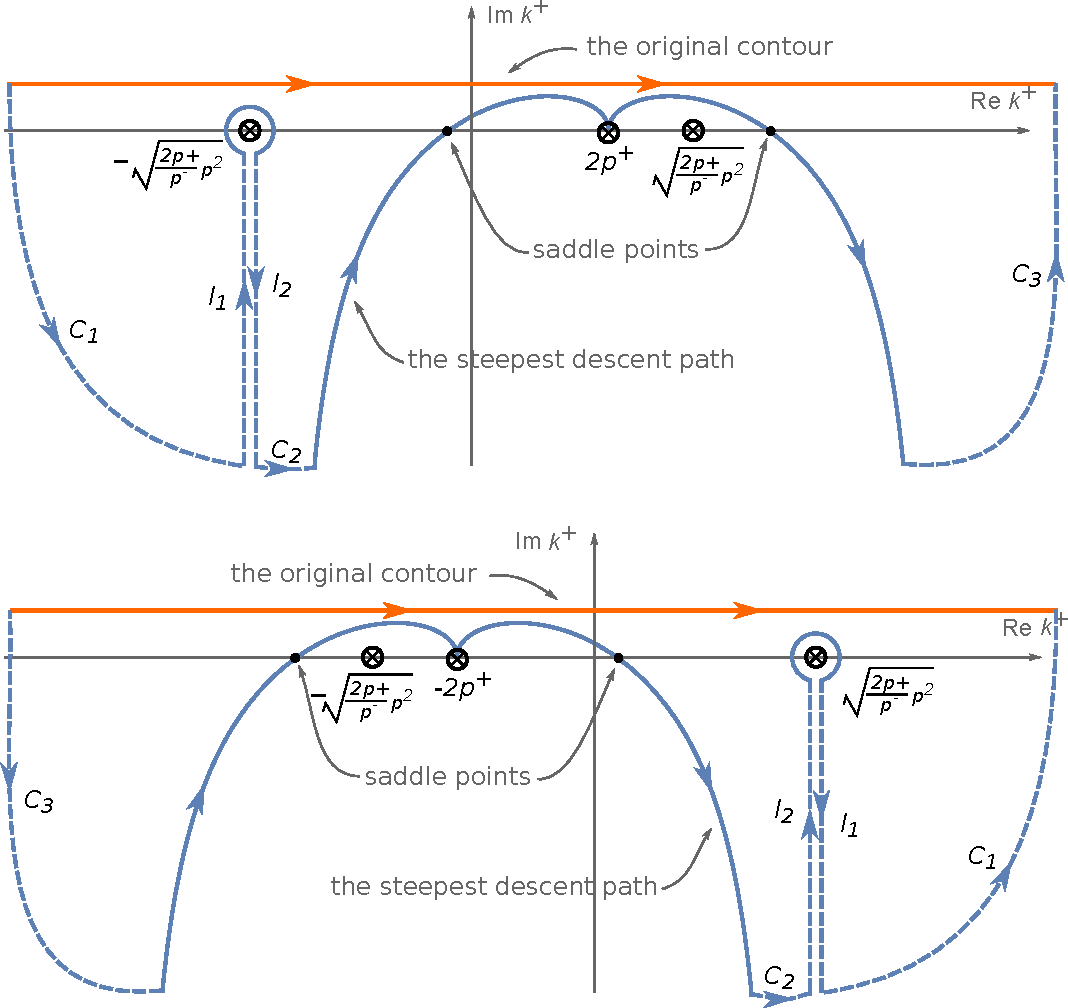
\includegraphics[width=0.55\textwidth]{fig/GXpLO}\\
\vspace{4mm}
{\tiny  {\color{teablue} Kovchegov \& BW,
  %``Kinetic transport is needed to reliably extract shear viscosity from pA and AA data,''
    JHEP {\bf 1803}, 157 \& 178 (2018).
  }
  }\\
  \vspace{2mm}
  {\color{darkred} $v_2$ can be calculated using the framework in these papers (working in progress).}
\end{center}
\end{frame}
\end{document}


